\chapter{UCNA Results}
\label{ch:UCNA_Results}
%%%%%%%%%%%%%%%%%%%%%%%%%%%%%%%%%%%%%%%%%%%%%%%%%%%%%%%%%%%%%%%%%%%%%%%%%%%%%%%
%%%%%%%%%%%%%%%%%%%%%%%%%%%%%%%%%%%%%%%%%%%%%%%%%%%%%%%%%%%%%%%%%%%%%%%%%%%%%%%
%%%%%%%%%%%%%%%%%%%%%%%%%%%%%%%%%%%%%%%%%%%%%%%%%%%%%%%%%%%%%%%%%%%%%%%%%%%%%%%


\section{Constructing an Asymmetry} \label{sec:asymmetry}

\subsection{Decay Rate Model}
As discussed in earlier in section \ref{ssec:neutronAsymmParam},
the nominal decay rate for polarized neutrons with no detection of
final-state spins is expressed in terms of the spin
vector of the neutron and all possible correlations to the products \cite{jackson1957a}.
For simplicity,
we begin by writing the differential decay rate for the case where only the electron
momentum is detectable (and assuming no BSM terms): 
%
\begin{equation} \label{eq:simpleRate}
\Gamma\left(E,\Omega\right)=C \cdot S(E) \cdot \big( 1+A(E)\beta\cos\theta \big),
\end{equation}
%
\noindent where $S(E)$ is the Standard Model differential decay rate for unpolarized
$\beta$-decay, $C$
is a constant which encompasses anything not included in $S(E)$ and serves the 
purpose of absorbing other constants, $A(E)$ is the 
energy dependent electron asymmetry parameter, $\beta\equiv v/c$ is the electron
velocity, and 
$\theta$ is the angle between the spin of the neutron and the electron momentum.

We can also introduce an average polarization of the neutrons, giving
%
\begin{equation}
  \Gamma\left(E,\Omega\right)=C \cdot S(E) \cdot \epsilon \cdot
  \big( 1+ \langle P \rangle\cdot A(E)\beta\cos\theta \big),
\end{equation}
%
\noindent where $\epsilon$ is the loading efficiency of neutrons
in this spin state which I haven't absorbed
into the constant for reasons to be seen, and 
$\langle P \rangle$ is the polarization, i.e. a number between 0 and 1 (very close to 1
in our case).

At this point, assumptions can be made regarding the experimental setup utilized
to further express the decay rate in terms of detector rates. Due to the spins
being aligned with the 1 T magnetic field in the decay trap, electrons emitted with
a momentum component along the spin will spiral towards one detector, while electrons
with a component of momentum opposite the spin will be detected in the opposite 
detector. If we fix the $z$-axis using the static position of our
apparatus, we can call the detector at $\theta=0$ detector
1 and the opposite detector 2. 

Now, all electrons with $0 < \theta < \pi/2$ will head towards detector 1 and those 
with $\pi/2 < \theta < \pi$ will be directed towards detector 2. The solid angle can
then be integrated out for each detector by integrating $\phi$ from $(0,2\pi)$ and
$\cos\theta$ over the intervals given, where the integral of $\cos\theta$ over detectors
1 and 2 yields $+1/2$ and $-1/2$ respectively: 
%
\begin{equation} 
  \Gamma_{1,2}\left(E\right)= 2\pi \cdot C \cdot S(E) \cdot
  \epsilon \cdot \eta_{1,2}(E) \left[ 1+ \langle P \rangle\cdot A(E)\beta
    \left(\pm_{1,2}\frac{1}{2}\right) \right],
\end{equation} 
%
\begin{equation} 
  \Gamma_{1,2}\left(E\right)=C' \cdot S(E) \cdot \epsilon \cdot \eta_{1,2}(E)
  \left[ 1 \pm_{1,2} \langle P \rangle\cdot A(E) \frac{\beta}{2} \right],
\end{equation} 
%
\noindent with $\eta_{1,2}(E)$ signifying energy dependent electron
detection efficiencies for detectors 1 and 2. 

Thus far we have assumed a fixed polarization, but in UCNA we have the ability to 
flip the spin of the neutrons prior to loading. We call these states flipper on ($+$) 
and flipper off ($-$), denoted by $\langle P \rangle_{\pm}$. The flipper on state introduces a
negative in front of the polarization efficiency
due to the fact that the spin $\vec{\sigma}$ is now aligned with $-\hat{z}$, thus reversing the sign
of $\vec{\sigma}\cdot\vec{p_{e}}$ with respect to the prior assumption of $\vec{\sigma}$ in $+\hat{z}$:
%
\begin{equation}
  \Gamma_{1,2}^{\pm}\left(E\right)=C' \cdot S(E) \cdot \epsilon_{\pm} \cdot \eta_{1,2}
  \left[ 1 \pm_{1,2} 
\left(\mp \langle P \rangle_{\pm}\right) \cdot A(E) \frac{\beta}{2} \right],
\end{equation} 
%
\noindent where $\epsilon_{\pm}$ accounts for differing loading efficiencies for 
different spin states.

If we now assume that we are equally as efficient at polarizing in either spin state, we
can say $\langle P \rangle_{+}=\langle P \rangle_{-}=\langle P \rangle$
(extraction of the asymmetry under the super-ratio technique not assuming this
condition can be found later in Section \ref{ssec:polSep}) giving:
%
\begin{equation} \label{eq:decayRate}
  \Gamma_{1,2}^{\pm}\left(E\right)=C' \cdot S(E) \cdot \epsilon_{\pm} \cdot \eta_{1,2}
  \left[ 1 \pm_{1,2} 
    \left(\mp \langle P \rangle \right) \cdot A(E) \frac{\beta}{2} \right].
\end{equation}
%

\subsection{Super-Ratio}

A simple asymmetry over some energy bin for a single 
polarization state can be defined as
%
\begin{equation} 
A_{\mathrm{simple}} = \frac{\Gamma_1 - \Gamma_2}{\Gamma_1 + \Gamma_2}, 
\end{equation}
%
\noindent and assuming that the efficiencies $\eta_1$ and $\eta_2$ are the same one
finds
%
\begin{equation} \label{eq:Asimple}
A_{\mathrm{simple}} = \langle P \rangle \cdot A(E) \cdot \frac{\beta}{2},
\end{equation}
%
\noindent where $\beta$ is calculated as either the velocity associated with the energy 
at the center of the bin or the average energy of the bin. The distinction is
unimportant as this is later corrected for as part of the angular acceptance correction
detailed in Section \ref{sssec:cosThetaCorr}.

In reality we cannot assume with certainty that the detectors are identical, but we can 
utilize the fact that we can flip the spins to cancel differing efficiencies. If we 
take two runs with opposite polarizations, we can define the super-ratio asymmetry in 
some energy range as:
%
\begin{equation} \label{eq:A_SR_frac}
A_{\mathrm{SR}} = \frac{1-\sqrt{R}}{1+\sqrt{R}} ,
\end{equation}
\noindent where 
\begin{equation} \label{eq:R}
 R = \frac{\Gamma_{1}^+ \cdot \Gamma_{2}^-}{\Gamma_{1}^- \cdot \Gamma_{2}^+}.
\end{equation}

Some algebra yields an identical expression to Equation \ref{eq:Asimple},
%
\begin{equation*}
R = \frac{ \left[ C'  S(E)  \epsilon_{+}  \eta_{1} \left[ 1 + 
      \left(- \langle P \rangle \right)  A(E) \frac{\beta}{2} \right] \right] 
\left[ C'  S(E)  \epsilon_{-}  \eta_{2} \left[ 1 - 
    \left(+ \langle P \rangle \right)  A(E) \frac{\beta}{2} \right] \right] }
{ \left[ C'  S(E)  \epsilon_{-}  \eta_{1} \left[ 1 + 
      \left(+ \langle P \rangle \right)  A(E) \frac{\beta}{2} \right] \right] 
\left[ C'  S(E)  \epsilon_{+}  \eta_{2} \left[ 1 - 
    \left(- \langle P \rangle \right)  A(E) \frac{\beta}{2} \right] \right] },
\end{equation*}
%
\begin{equation*}
R = \frac{ \left[ 1 + \left(- \langle P \rangle \right)  A(E) \frac{\beta}{2} \right] 
\left[ 1 - \left(+ \langle P \rangle \right)  A(E) \frac{\beta}{2} \right]  }
{  \left[ 1 +  \left(+ \langle P \rangle \right)  A(E) \frac{\beta}{2}  \right] 
 \left[ 1 -  \left(- \langle P \rangle \right)  A(E) \frac{\beta}{2} \right]},
\end{equation*}
%
\begin{equation*}
R = \frac{ \left[ 1 -  \langle P \rangle  A(E) \frac{\beta}{2} \right]^2 }
{  \left[ 1 + \langle P \rangle  A(E) \frac{\beta}{2}  \right]^2 },
\end{equation*}
%
\noindent and plugging into $A_{\mathrm{SR}}$
%
\begin{equation*}
  A_{\mathrm{SR}} = \frac{1-\frac{ \left[ 1 -  \langle P \rangle  A(E) \frac{\beta}{2} \right] }
{  \left[ 1 + \langle P \rangle  A(E) \frac{\beta}{2}  \right] } }
  {1+\frac{ \left[ 1 -  \langle P \rangle  A(E) \frac{\beta}{2} \right] }
{  \left[ 1 + \langle P \rangle  A(E) \frac{\beta}{2}  \right] }},
\end{equation*}
%
\begin{equation*}
A_{\mathrm{SR}} = \frac{2 \langle P \rangle A(E) \frac{\beta}{2}}{2},
\end{equation*}
%
\begin{equation} \label{eq:A_SR}
A_{\mathrm{SR}} = \langle P \rangle A(E) \frac{\beta}{2}.
\end{equation}

The super-ratio not only cancels the detector efficiencies, but any difference between the
integrated rates between the two spin states also cancel.

\subsection{Extracting $A_0$}

The quantity of interest is not the raw measured asymmetry, or even $A(E)$,
but rather $A_0$, which is directly proportional to $\lambda=g_A/g_V$, yielding a direct 
measurement of the axial vector coupling constant if the CVC hypothesis is assumed. 

$A_0$ manifests itself in our measured asymmetry as:
%
\begin{equation}
A_0 = A(E) \cdot \left( 1 + \Delta(E) \right),
\end{equation}
%
\noindent where $\Delta(E)$ is the energy dependent correction to the measured asymmetry
from theory corrections and experimental systematic effects, all of which will be
described in detail in \ref{sec:systematics}. The modifications from theory were
also mentioned in chapter 1.

Solving \ref{eq:A_SR} for $A(E)$ and inserting into the above expression, we have 
%
\begin{equation}
  A_0 = \frac{\big( 1 + \Delta(E) \big) \cdot A_{\mathrm{SR}}(E) }
  {\langle P \rangle \cdot \beta/2},
  \label{eq:A0}
\end{equation}
%
\noindent where again $\beta=v/c$. 

With an energy dependent expression for $A_0$, we can bin our data in discrete
energy bins, evaluate $\beta$ at the midpoint of the bin, apply appropriate energy
dependent corrections, and then fit the resulting collection of $A_0$ values with a
constant. Careful selection of the energy range to fit over is discussed
in \ref{ssec:enRange}. 


%--------------------------------------------------------------------------------------------------
\section{Systematic Corrections and Uncertainties} \label{sec:systematics}

Measuring any quantity without imparting a systematic shift in the result due to
imperfect experimental techniques is nearly impossible; but what is more dangerous
to the result is not understanding these shifts. This section discusses how well
we understand the theoretical and experimental effects present in the UCNA
experiment that cause us to measure an asymmetry that is not directly equal to
the parameter of interest, thus requiring corrections.

\subsection{Definition of $\Delta$}

We adopt a similar formalism for systematic corrections as previously defined in
\cite{mpmThesis}, at least as far as the definition of the correction is concerned.
If we have an asymmetry $A(E)$ measured without some correction $i$,
then we can define $A'(E)$ as
%
\begin{equation} \label{eq:aprimedelta}
  A'(E) = \big( 1 + \Delta_i(E) \big) \cdot A(E),
\end{equation}
%
\noindent where $A'(E)$ is the new corrected asymmetry with systematic effect $i$ removed.
Rearrangement of the above equation provides a definition for $\Delta_i$:
%
\begin{equation} \label{eq:delta}
  \Delta_i(E) = \frac{A'(E)}{A(E)} - 1
\end{equation}
%
This is useful as most corrections are determined by studying the effect on the asymmetry
from some aspect of the experiment via Monte Carlo, so energy dependent corrections can
be constructed and applied to data.

If the uncertainty on correction $\delta\Delta_i$, denoted $\delta \Delta_i$,
has been determined, we can also define
the uncertainty on the resulting asymmetry $\delta A'(E)$ via normal error propagation
techniques as
%
\begin{equation} 
  \delta A'(E) = A(E) \cdot \delta\Delta_i(E),
\end{equation}
%
\begin{equation} 
  \frac{\delta A'(E)}{A'(E)} =  \frac{ \delta\Delta_i(E)}{1+\Delta_i(E)}.
\end{equation}

Now the collection of all corrections, if extracted independently, will commute, and thus
provides
%
\begin{equation}
1+\Delta(E)=\big(1+\Delta_1(E)\big)\big(1+\Delta_2(E)\big)\big(1+\Delta_3(E)\big)\ldots,
\end{equation}
%
\noindent such that a final corrected asymmetry $A'''^{\ldots}$ can be written as 
%
\begin{equation*}
A'''^{\ldots}(E) = \big(1+\Delta(E)\big) \cdot A(E),
\end{equation*}
%
\begin{equation}
A'''^{\ldots}(E) = \Big(\prod_i\big(1+\Delta_i(E)\big)\Big)\cdot A(E).
\end{equation}

The rest of this section is dedicated to determining all applicable $\Delta_i$
and their associated uncertainties.

\subsection{Energy Dependent Monte Carlo Corrections}

The Monte Carlo corrections are calculated by forming asymmetries from simulated data with
the entirety of the detector response model applied. For each individual data run, the
conditions of the apparatus (calibration, pedestal, resolution, etc) are determined
and a subset of the simulation data (roughly $16 \times $ the data run) is processed
using such conditions. This produces a higher statistics simulation of the individual runs,
and therefore allows one to run the simulated octets through the asymmetry analysis in
the exact same manner as the data. The fact that we know everything about each individual
event in the simulation allows us to correct for effects to the asymmetries from
the experimental conditions. Via Equation \ref{eq:delta}, the asymmetry before and after
a given correction can be used to determine the value of the correction to be applied to the
data.

The Monte Carlo corrections are also further separated into corrections from misidentification
of backscattering types, $\Delta_{2}$, and from angular acceptance effects, $\Delta_{3}$.
In \cite{brown2017}, $\Delta_{2}$ and $\Delta_{3}$ correspond to $\Delta_{\mathrm{backscattering}}$ and
$\Delta_{\mathrm{\cos\theta}}$ respectively.

\subsubsection{Backscattering Misidentification, $\Delta_{2}$}
Imagine an event which initially heads towards the east detector, but it backscatters
off of the decay trap window and never reaches a sensitive detector on the East side. The
electron then heads towards the West detector where it is detected. Using only triggering
information, this event would be improperly identified as a Type 0 event with initial Western
momentum. Experimental data possess no way of properly identifying such events, so we rely
on simulation. As mentioned previously, we have access to all initial conditions of each simulated event,
so upon forming an asymmetry one can properly identify all events which were detected as Type 0
and assure they are assigned to their proper initial direction. The comparison of the asymmetry
before and after such a correction defines the Monte Carlo correction due to backscattering
misidentification of Type 0 events. Let's call this $\Delta_{2,0}$, where the subscript 0 refers
to the backscattering correction for Type 0 events. One can imagine that the same process can
be repeated for each of the detected event types, giving us the following definition for
the total $\Delta_{2}$ correction:
%
\begin{equation}
1+\Delta_{2} = (1+\Delta_{2,3})(1+\Delta_{2,2})(1+\Delta_{2,1})(1+\Delta_{2,0})
\end{equation}



\begin{figure}[p]
  \centering
  \captionsetup{justification=centering} 
  \begin{tabular} {cc}
    \subfloat[~~2011-2012:~$0.71(26)\%$\newline2012-2013:~$0.51(26)\%$]{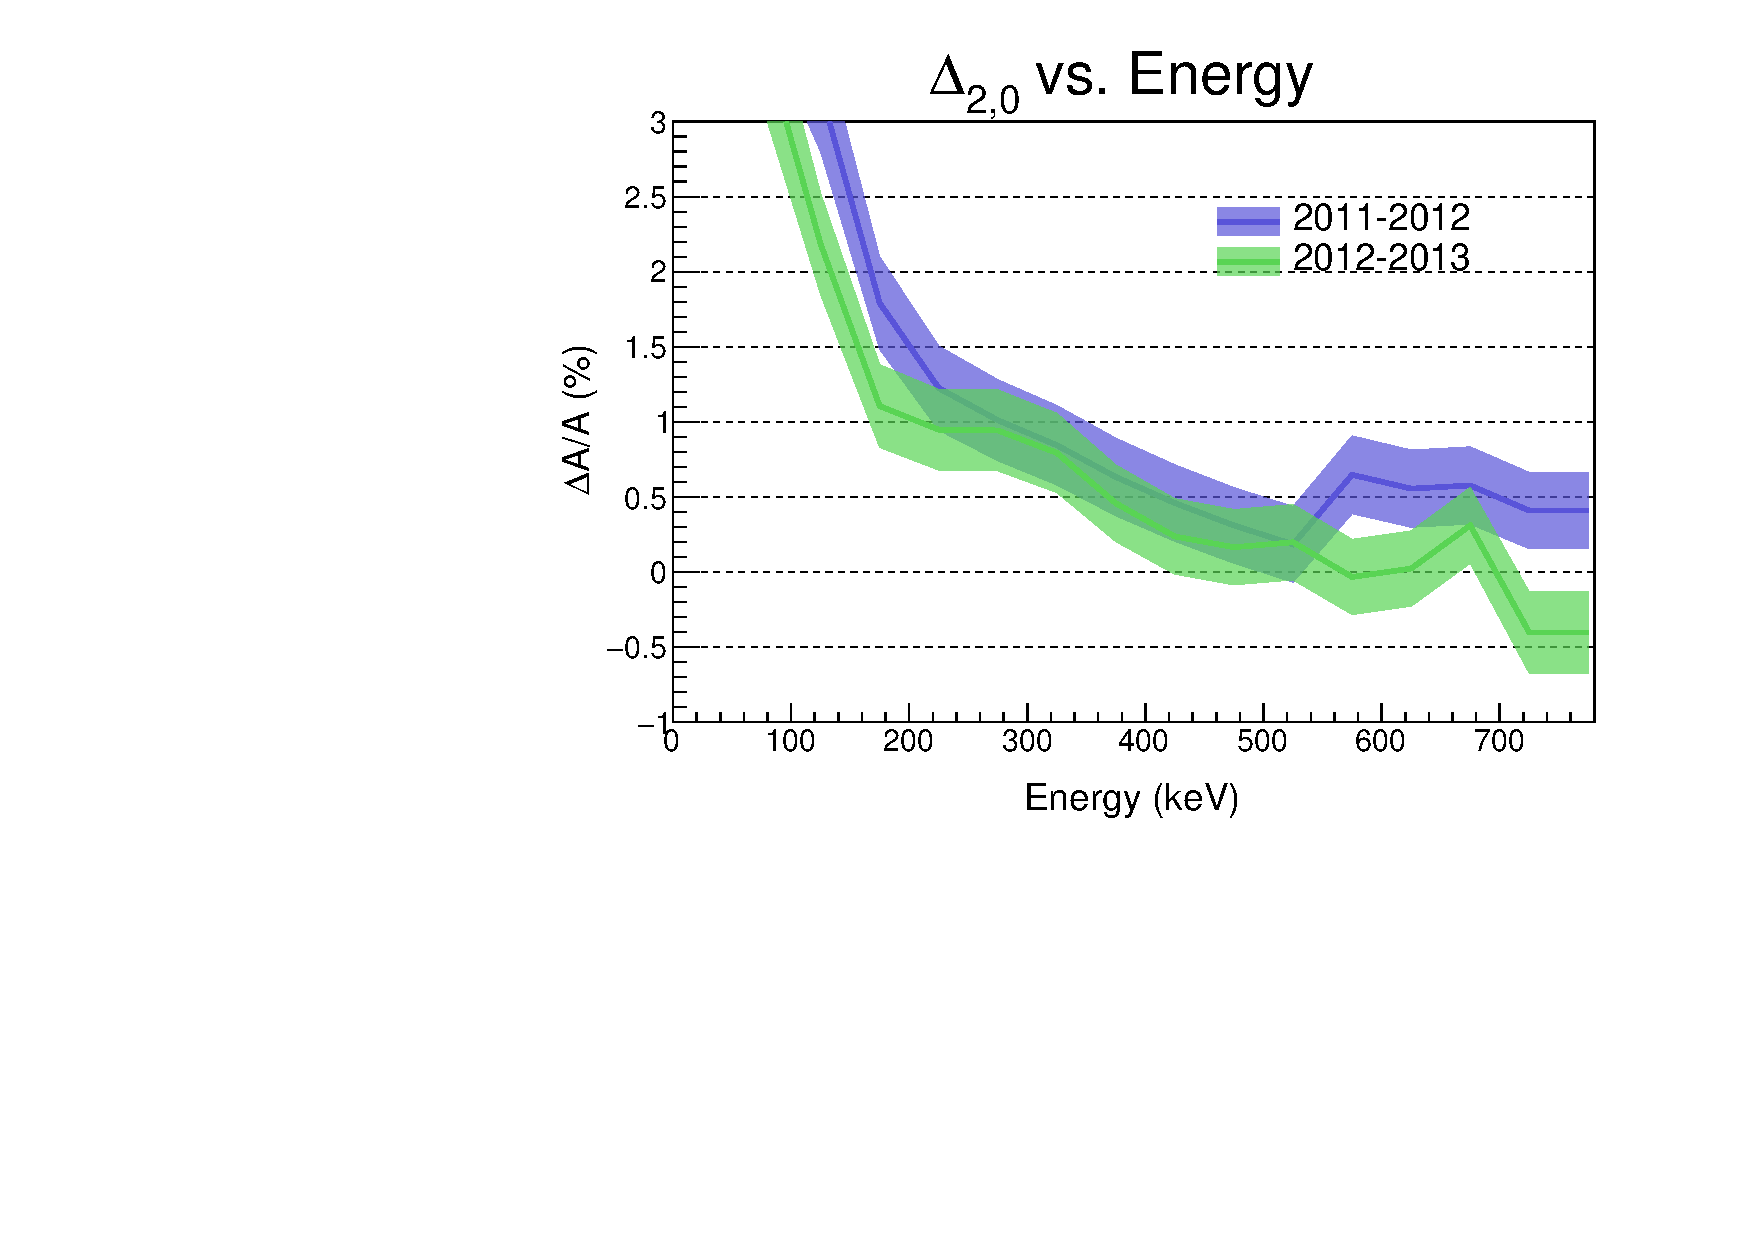
\includegraphics[page=1,scale=0.35]{5-UCNAResults/Delta_2_byType_anaChC_5BinAve_color.pdf}}&
    \subfloat[~~2011-2012: $0.05(8)\%$\newline2012-2013: $0.04(8)\%$]{\includegraphics[page=2,scale=0.35]{5-UCNAResults/Delta_2_byType_anaChC_5BinAve_color.pdf}}
  \end{tabular}
  \begin{tabular} {cc}
    \subfloat[~~2011-2012: $0.14(9)\%$\newline2012-2013: $0.15(10)\%$]{\includegraphics[page=3,scale=0.35]{5-UCNAResults/Delta_2_byType_anaChC_5BinAve_color.pdf}}&
    \subfloat[~~2011-2012: $0.19(8)\%$\newline2012-2013: $0.18(08)\%$]{\includegraphics[page=4,scale=0.35]{5-UCNAResults/Delta_2_byType_anaChC_5BinAve_color.pdf}}
  \end{tabular}
  \subfloat[~~2011-2012: $1.08(30)\%$\newline2012-2013: $0.88(31)\%$]{\includegraphics[page=5,scale=0.35]{5-UCNAResults/Delta_2_byType_anaChC_5BinAve_color.pdf}}
  \captionsetup{justification=justified} 
  \caption{Backscattering corrections for analysis choice used in final asymmetry extraction
    (All event types included with 2/3 separated using
    the MWPC energy calibration). The corrections reported in the captions are integrated over the final
    analysis window $190\mathrm{~keV}<T_e<740\mathrm{~keV}$, the determination of which will be discussed in Section \ref{ssec:enRange}.}
  \label{fig:delta2}
\end{figure}

The corrections as a function of electron energy can be seen in figure
\ref{fig:delta2}.  Application of the correction increases
the magnitude of the measured asymmetry as it should, as missed backscattering events
dilute the measured asymmetry. The uncertainties seen in the figure
will be discussed in Section \ref{sssec:mcuncert}.
The leading contribution to the backscattering correction
comes from Type 0 events due to them accounting for roughly
$95\%$ of the data. The other event types have much smaller contributions to
the backscattering correction when all event types are included in the analysis
due primarily to the little statistical weight they carry. If the Type 0 events
are ignored, the backscattering corrections become very large for the Type 1, 2,
and 3 events. This will be illustrated when showing asymmetries for different
combinations of event types later in this chapter.


\begin{figure}[h]
  \centering
  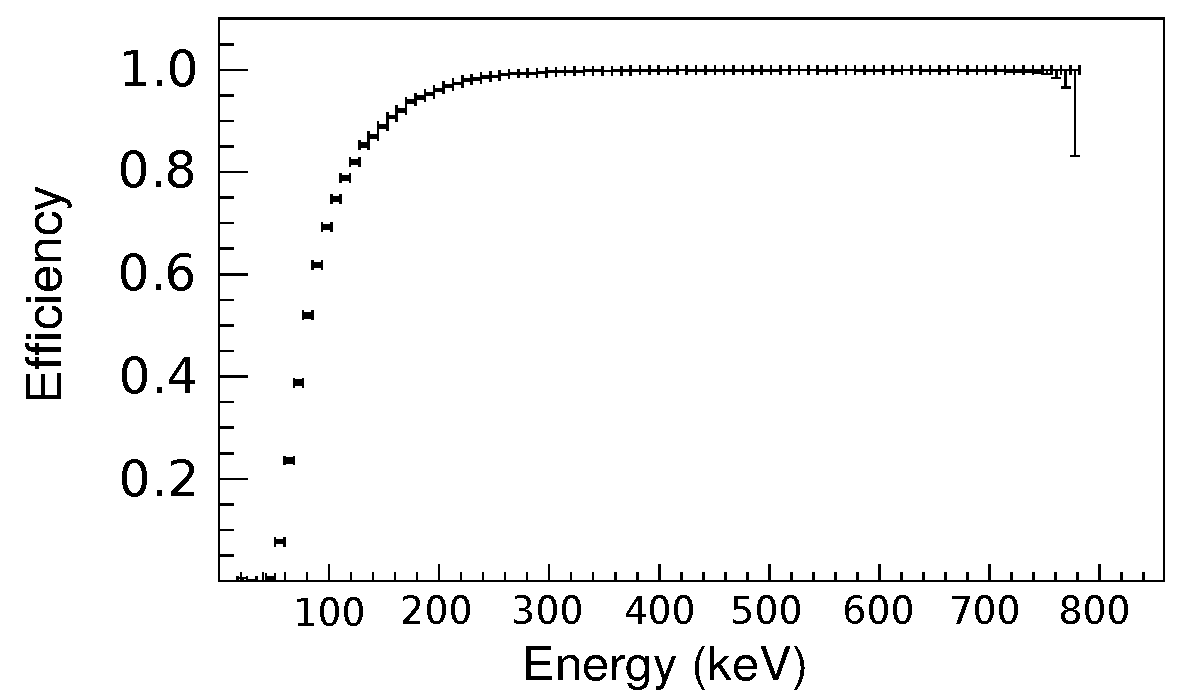
\includegraphics[scale=0.40]{5-UCNAResults/efficiency.pdf}  
  \caption{Simulated detector efficiency as a function of electron energy for electrons which
  pass through the decay trap endcaps.}
  \label{fig:effic}
\end{figure}

The difference between 2011-2012 and 2012-2013 corrections arises from the thinner
decay trap windows in 2012-2013, which substantially reduces the $\Delta_{2,0}$
correction for
misidentified Type 0 events. There is almost no effect on the other event types, as should
be expected due to no dramatic change in event type fractions or triggering efficiencies
for the two detector sides. Another way to think of this is that once an event passes through the
decay trap endcap, it's likelihood of triggering the detector approaches $100\%$ fairly quickly
(see Figure \ref{fig:effic}) and is not dependent on the changing geometry, so the corrections for
backscattering events are robust. Differing endcap thicknesses do however modify the number of misidentified
Type 0 events, decreasing them in the case of thinner windows as more electrons should pass through without
scattering, thus decreasing the magnitude of the
$\Delta_{2,0}$ correction by definition.


\subsubsection{Angular Acceptance, $\Delta_{3}$} \label{sssec:cosThetaCorr}
Remember from Equation \ref{eq:simpleRate} that the asymmetric
component of the decay rate depends on
$\beta\cos\theta$ and that we proceeded to integrate over one hemisphere
of the detector giving $\langle\cos\theta\rangle=1/2$. We also use the midpoint
of the energy bin of interest when evaluating $\beta=v/c$, which isn't equal to the
average value in a single bin due to the non-constant shape of the electron energy
spectrum. What is described is
an approximation of the form $\langle\beta\cos\theta\rangle \approx \beta_{\mathrm{mid}}/2$. The actual
value of $\langle\beta\cos\theta\rangle$ must be determined using simulated
data, as events are lost in an energy and angle dependent manner, with lower energy and
high pitch angle events being most likely to be lost. $\Delta_{3}$ attempts to
remove this angular dependence on event acceptance while also correcting for the slight
systematic effect of approximating $\beta$ at the midpoint.

If we define the asymmetry which properly accounts for the true $\langle\beta\cos\theta\rangle$
as $A'$ and the asymmetry which uses our approximation
$\langle\beta\cos\theta\rangle \approx \beta_{\mathrm{mid}}/2$ as $A$, then we see from
\ref{eq:A_SR} that
%
\begin{equation} \label{eq:ap}
  A' = \frac{A_{\mathrm{SR}}}{\langle\beta\cos\theta\rangle \langle P \rangle}
\end{equation}
%
\noindent and
%
\begin{equation} \label{eq:a}
  A = \frac{A_{\mathrm{SR}}}{\frac{\beta}{2} \langle P \rangle}.
\end{equation}
%
\noindent Then from our generic definition for a systematic correction, equation
\ref{eq:delta}, we have
%
\begin{equation*}
\Delta_3(E) = \frac{A'}{A}-1
\end{equation*}
%
\noindent and upon use of equations \ref{eq:ap} and \ref{eq:a},
%
\begin{equation} \label{eq:delta3def}
\Delta_3(E) = \frac{\frac{\beta}{2}}{\langle\beta\cos\theta\rangle}-1\textrm{ .}
\end{equation}
%
\noindent From this, we see that it is sufficient to determine $\langle\beta\cos\theta\rangle$
from simulation and calculate the energy dependent corrections.

\begin{figure}[p]
  \centering
  \captionsetup{justification=centering} 
  \begin{tabular} {cc}
    \subfloat[~~2011-2012: $-2.46(25)\%$\newline2012-2013: $-2.41(25)\%$]{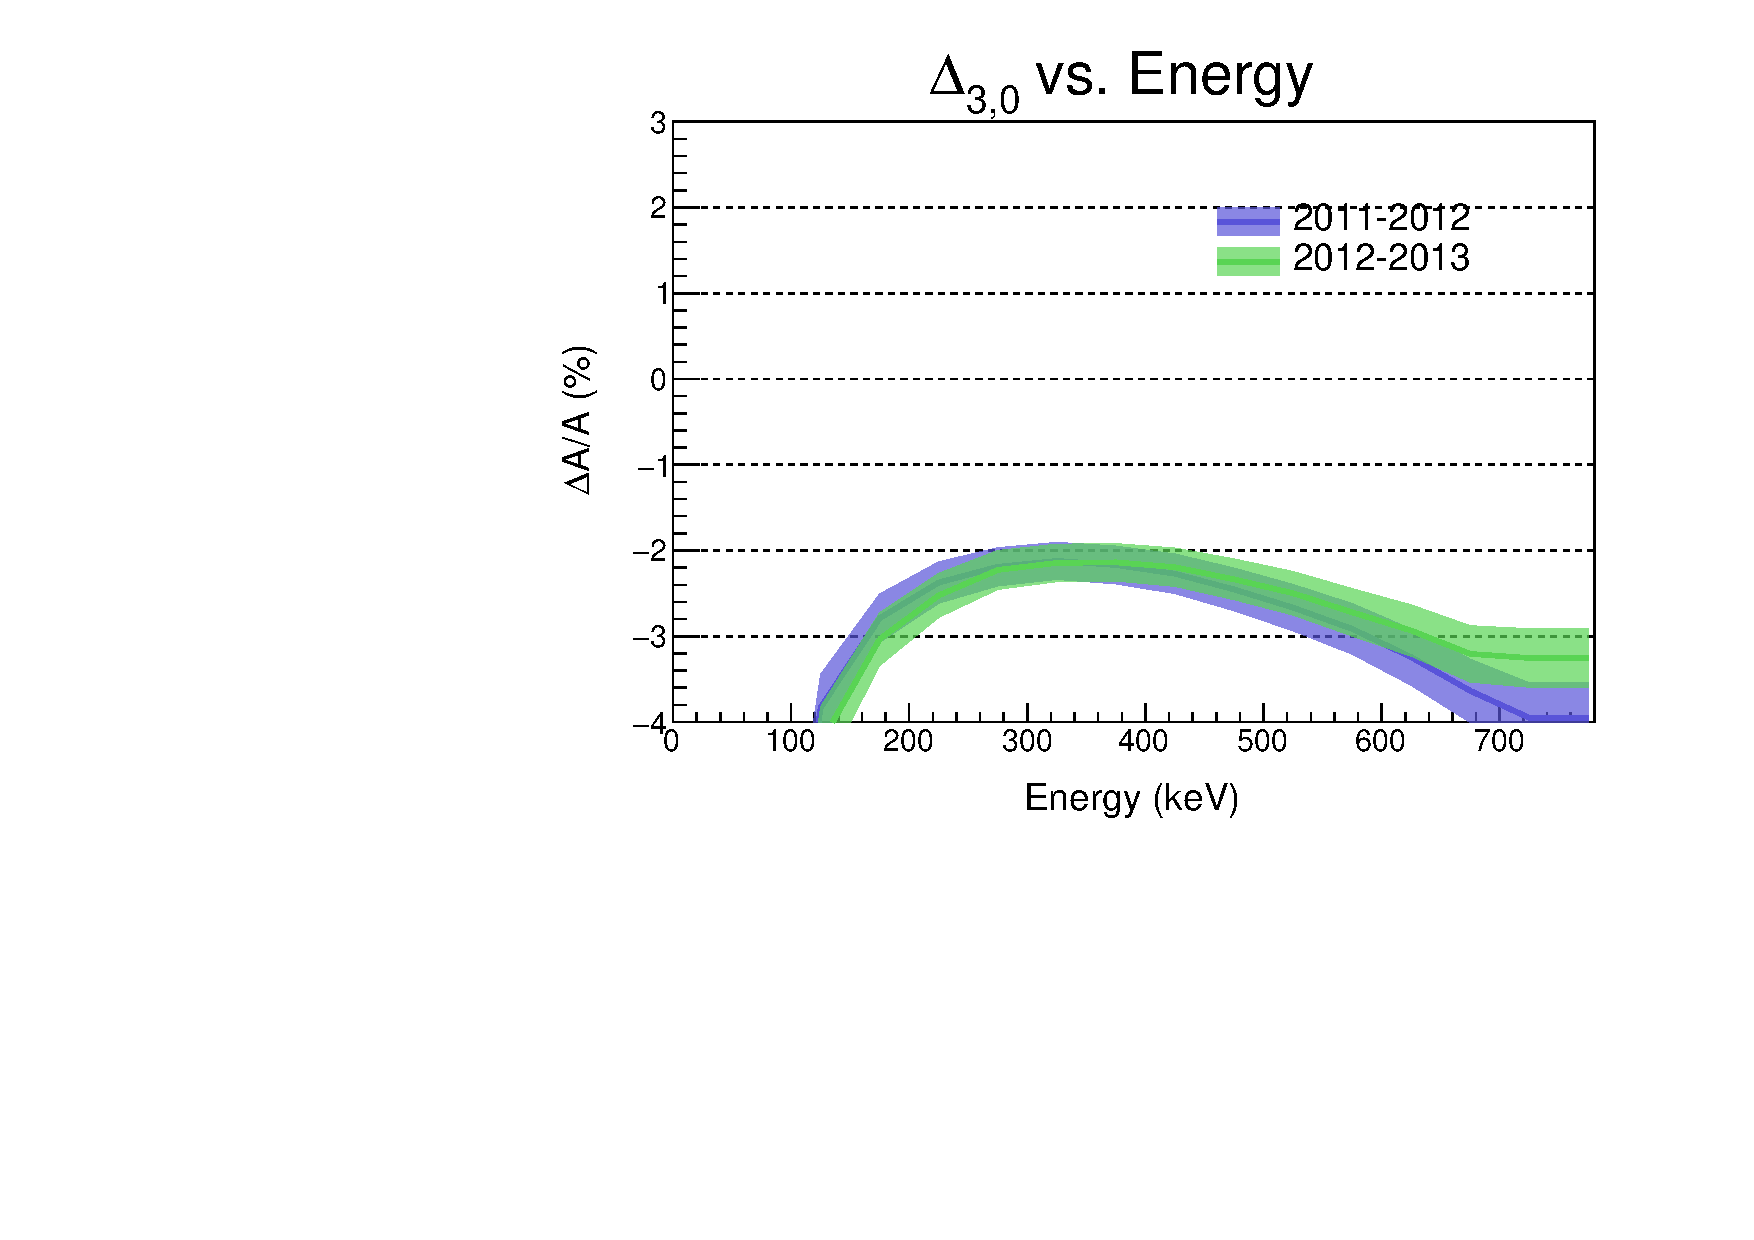
\includegraphics[page=1,scale=0.35]{5-UCNAResults/Delta_3_byType_anaChC_5BinAve_color.pdf}}&
    \subfloat[~~2011-2012: $0.66(21)\%$\newline2012-2013: $0.64(20)\%$]{\includegraphics[page=2,scale=0.35]{5-UCNAResults/Delta_3_byType_anaChC_5BinAve_color.pdf}}
  \end{tabular}
  \begin{tabular} {cc}
    \subfloat[~~2011-2012: $0.12(6)\%$\newline2012-2013: $0.11(5)\%$]{\includegraphics[page=3,scale=0.35]{5-UCNAResults/Delta_3_byType_anaChC_5BinAve_color.pdf}}&
    \subfloat[~~2011-2012: $0.13(4)\%$\newline2012-2013: $0.14(4)\%$]{\includegraphics[page=4,scale=0.35]{5-UCNAResults/Delta_3_byType_anaChC_5BinAve_color.pdf}}
  \end{tabular}
  \subfloat[~~2011-2012: $-1.53(33)\%$\newline2012-2013: $-1.51(33)\%$]{\includegraphics[page=5,scale=0.35]{5-UCNAResults/Delta_3_byType_anaChC_5BinAve_color.pdf}}
  \captionsetup{justification=justified} 
  \caption{$\cos\theta$ corrections for analysis choice used in final asymmetry extraction
    (All event types included with 2/3 separated using
    the MWPC energy calibration). The corrections reported in the captions are integrated over the final
  analysis window $190\mathrm{~keV}<T_e<740\mathrm{~keV}$, the determination of which will be discussed in Section \ref{ssec:enRange}.}
  \label{fig:delta3}
\end{figure}
%
%\begin{figure}[h]
%  \centering
%  \includegraphics[page=7,scale=0.35]{5-UCNAResults/Delta_2_byType_anaChC_5BinAve_color.pdf}
%  \caption{Here is a caption}
%  \label{fig:deltaMC}
%\end{figure}
%

In previous analyses, this correction was done for the event population as a whole, producing
only a single correction $\Delta_3$. New work specific to this thesis allows for
separation of this correction into individual contributions from each event type,
%
\begin{equation}
1+\Delta_{3} = (1+\Delta_{3,3})(1+\Delta_{3,2})(1+\Delta_{3,1})(1+\Delta_{3,0}).
\end{equation}
%
\noindent This is more difficult than separating $\Delta_2$, as it requires more than a simple
event-by-event reassignment to the proper initial direction. This requires evaluation of
an average observable in the simulation, so we need a way to realize the contribution
of each event type to the average. The key is to use the individual asymmetry of each event
type and its respective angular correction, and then define the total correction as a function
of the individual corrections. 

Determination of the $\Delta_{3,i}$ corrections starts with a new definition of the
uncorrected combined asymmetry\footnote{\label{fnote:newAsymmDef}This definition
of the asymmetry is only used for analysis of this correction, and not for extraction
of the final asymmetry.} involving the individual asymmetries of each event type.
The following definitions will be useful in this derivation.
%
\begin{align*}
  &A \equiv \textrm{Uncorrected total asymmetry}\\
  &A^i \equiv \textrm{Asymmetry for event type } i\\
  &f^i \equiv \textrm{Statistical weight for event type }i\\
  &\Delta^i_3 \equiv \textrm{Angle correction to }A^i\textrm{ for event type }i\\
  &A^{\mathrm{corr},i} \equiv \textrm{Corrected asymmetry for event type } i\\
  &A_{\mathrm{corr},i} \equiv \textrm{Total asymmetry corrected for event type } i\\
  &\Delta_{3,i} \equiv \textrm{Angle correction to total asymmetry }A
  \textrm{ for event type }i
\end{align*}
%

Now we can define the uncorrected total asymmetry as
%
\begin{equation}
A=\sum_i f^iA^i
\end{equation}
%
\noindent where the sum runs over the event types that are to be included in the
determination of the asymmetry. As will be seen in \ref{sssec::anaChoices}, one can include
any combination of event types to produce many different asymmetries, so this definition
allows for use across any choice of event types.

Next we can define $\Delta^i_3$, or the angle correction to the asymmetry when only
including type $i$ events, using Equation \ref{eq:delta3def} and only including
type $i$ events when calculating $\langle\beta\cos\theta\rangle$. Then we can write down
an expression for the corrected asymmetry for that event type as
%
\begin{equation}
A^{\mathrm{corr},i} = (1+\Delta^i_3)A^i.
\end{equation}

It then follows that the total asymmetry corrected for the same event type $i$ becomes
%
\begin{equation}
A_{\mathrm{corr},i} = A^{\mathrm{corr},i} + \sum_{j\neq i} f^jA^j.
\end{equation}

With these relationships at hand, it is straightforward to follow the prescription to write
down an expression for $\Delta_{3,i}$ in terms of known values:
%
\begin{equation*}
  \Delta_{3,i} = \frac{A_{\mathrm{corr},i}}{A} - 1 = \frac{A_{\mathrm{corr},i}-A}{A} =
  \frac{f^i(A^{\mathrm{corr},i}-A^i)}{A}
\end{equation*}
%
\begin{equation}
  \Rightarrow\Delta_{3,i} = \frac{f^iA^i}{A}\Delta^i_3.
\end{equation}
%

The energy dependent $\Delta_{3,i}$ corrections are shown in Figure \ref{fig:delta3}.
The impact of applying the combined $\Delta_{3}$ correction is to decrease the magnitude of the
measured asymmetry. This comes from the dominance of the $\Delta_{3,0}$ portion, or the correction
due to the acceptance of Type 0 events. Type 0 events are more likely lost when they are high pitch
angle, low energy events. Such events carry little asymmetry information ($\beta\cos\theta$ gets small)
as seen in Equation \ref{eq:simpleRate}. Measurement of an asymmetry which has these low-asymmetry events
removed yields a larger magnitude asymmetry, thus necessitating a correction which decreases the
magnitude of the measured asymmetry. The contribution of the backscattering events to the angular
correction have the opposite sign and act to increase the magnitude of the measured asymmetry.
While this may seem counterintuitive due to the detectors nominally preferentially selecting
low pitch angle, high energy events, this sign is due to the backscattering events being overwhelmingly
high pitch angle events. Therefore $|\langle\cos\theta\rangle|$ over one hemisphere of the decay trap
will be less than the nominal value $1/2$ for all
backscattering events types, calling for a correction which increases the magnitude of the measured
asymmetry.

\subsubsection{Uncertainty in $\Delta_{\mathrm{MC}}$} \label{sssec:mcuncert}

In the analysis of the previous 2010 data set \cite{mendenhall2013} a
conservative 25\% uncertainty was applied to all Monte Carlo corrections, where the
25\% came from the observed discrepancy between data and Monte Carlo backscattering
fractions.  
The issue with such a correction is obvious when the correction itself is zero, as
any percent uncertainty on that correction would also be zero. One might argue that
the absence of a correction would imply the absence of an uncertainty in that correction,
but we must remember that the corrections are determined using Monte Carlo simulations
of finite statistics, thus even a 0\% correction comes with an uncertainty.
Another concern is that not all event type fractions disagree with Monte Carlo by
25\%, and the backscattering spectra that do disagree contribute little statistically
to the asymmetry. Also, the asymmetry is no longer dominated by statistical uncertainty,
and, as will be seen in Section \ref{ssec:energyRecon}, the uncertainty due to energy
reconstruction has been reduced, thus the ultra conservative worst-case scenario may
artificially limit our result.
With these  concerns taken into consideration, a new method was developed to assess
the uncertainty on the Monte Carlo corrections motivated by the fractional discrepancies
between data and simulation for each event type, denoted by $\delta_{\mathrm{frac}}\Delta_{i,j}$,
and the statistical fluctuations in the
corrections themselves, $\delta_{\mathrm{stat}}\Delta_{i,j}$.
%
\begin{figure}[h]
  \centering
  \begin{tabular} {cc}
    \subfloat[$\Delta_{2,0}$]{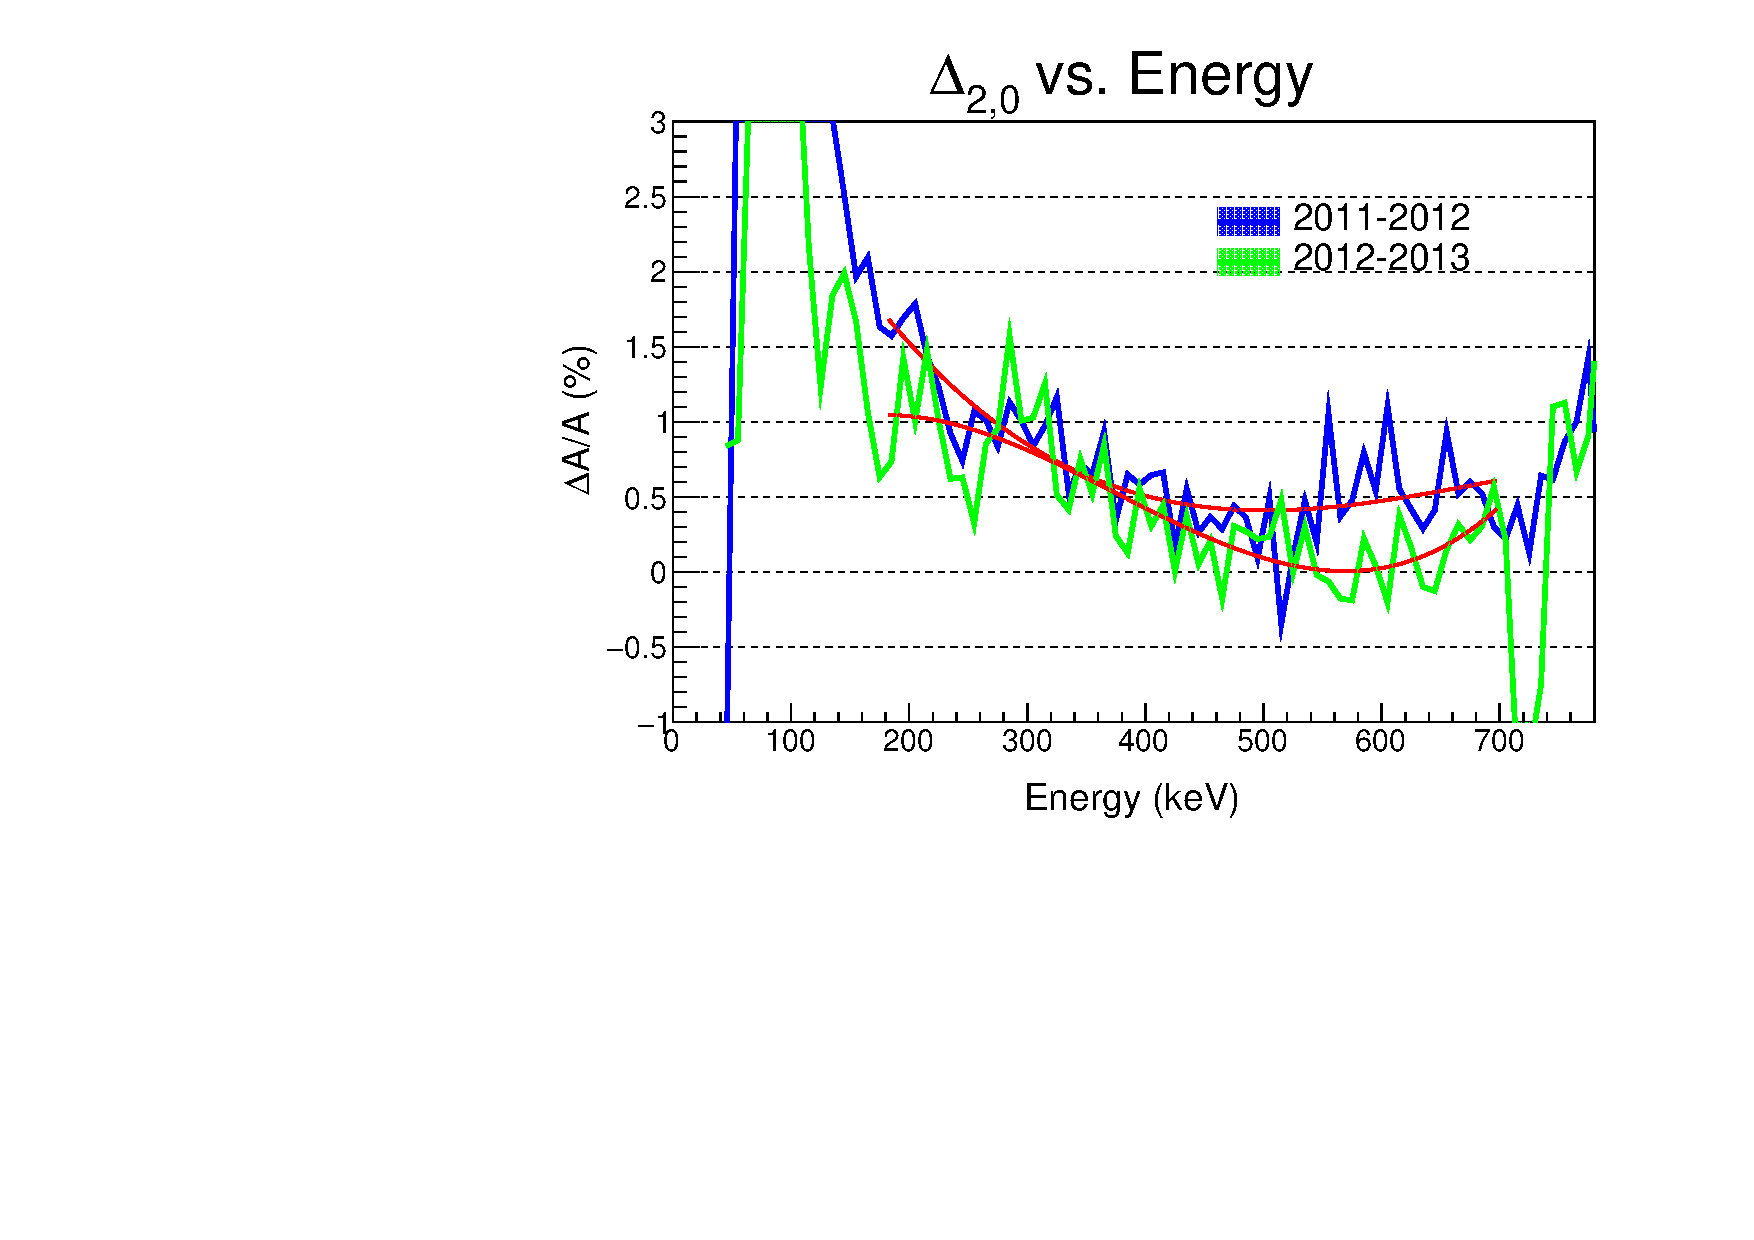
\includegraphics[page=1,scale=0.32]{5-UCNAResults/MC_Fits_anaChC.pdf}}&
    \subfloat[$\Delta_{2,1}$]{\includegraphics[page=2,scale=0.32]{5-UCNAResults/MC_Fits_anaChC.pdf}}
  \end{tabular}
  \begin{tabular} {cc}
    \subfloat[$\Delta_{2,2}$]{\includegraphics[page=3,scale=0.32]{5-UCNAResults/MC_Fits_anaChC.pdf}}&
    \subfloat[$\Delta_{2,3}$]{\includegraphics[page=4,scale=0.32]{5-UCNAResults/MC_Fits_anaChC.pdf}}
  \end{tabular}
  \caption{Bin-by-bin $\Delta_2$ corrections  with
    polynomial fit shown in red.}
  \label{fig:effStat}
\end{figure}
%
\begin{figure}[h]
  \centering
  \begin{tabular} {cc}
    \subfloat[$\Delta_{3,0}$]{\includegraphics[page=5,scale=0.32]{5-UCNAResults/MC_Fits_anaChC.pdf}}&
    \subfloat[$\Delta_{3,1}$]{\includegraphics[page=6,scale=0.32]{5-UCNAResults/MC_Fits_anaChC.pdf}}
  \end{tabular}
  \begin{tabular} {cc}
    \subfloat[$\Delta_{3,2}$]{\includegraphics[page=7,scale=0.32]{5-UCNAResults/MC_Fits_anaChC.pdf}}&
    \subfloat[$\Delta_{3,3}$]{\includegraphics[page=8,scale=0.32]{5-UCNAResults/MC_Fits_anaChC.pdf}}
  \end{tabular}
  \caption{Bin-by-bin $\Delta_3$ corrections with
    polynomial fit shown in red.}
  \label{fig:effStatDelta3}
\end{figure}

We further break up the statistical uncertainty
into two parts and add these in quadrature to get $\delta_{\mathrm{stat}}\Delta_{i,j}$.
There is an obvious uncertainty
that comes from simply propagating the statistics of the simulation through the correction,
which we will call
$\delta^{\mathrm{pure}}_{\mathrm{stat}}\Delta_{i,j}$.
This uncertainty doesn't seem to account for the fluctuations we see in the correction though, as
seen in Figure \ref{fig:effStat} panel (a) where the correction, when plotted for each
energy bin, oscillates at the roughly 0.25\% correction level at higher energies. This
oscillation may be due to correlations between the Monte Carlo events used to simulate each
run, as there are only 200 million events for each geometry and the events are chosen
randomly from this pool of events. Regardless of the cause, we account
for this observed statistical fluctuation using what we call the effective statistical
uncertainty, or $\delta^{\mathrm{eff}}_{\mathrm{stat}}\Delta_{i,j}$, which gives us
%
\begin{equation*}
  \delta \Delta_{i,j} = \sqrt{ (\delta_{\mathrm{frac}}\Delta_{i,j})^2 + ( \delta_{\mathrm{stat}}\Delta_{i,j})^2}
\end{equation*}
%
\begin{equation}
  \delta \Delta_{i,j} = \sqrt{ (\delta_{\mathrm{frac}}\Delta_{i,j})^2 +
    ( \delta^{\mathrm{pure}}_{\mathrm{stat}}\Delta_{i,j})^2 +
    ( \delta^{\mathrm{eff}}_{\mathrm{stat}}\Delta_{i,j})^2} .
\end{equation}

\setlength{\tabcolsep}{12pt}

\begin{table}[h]
  \caption{Values for the effective statistical uncertainties from each
  event type. The value is reported as the uncertainty on $\frac{\Delta A}{A}$.} 
  \centering
  \begin{tabular}{l c }
    \hline \hline \\ [-1.75ex]
    & \% Uncert. \\
    \hline \\ [-1.75ex]
    $\delta^{\mathrm{eff}}_{\mathrm{stat}}\Delta_{2,0}$ & $\pm0.25$ \\ [0.50ex]
    $\delta^{\mathrm{eff}}_{\mathrm{stat}}\Delta_{2,1}$ & $\pm0.074$ \\ [0.50ex]
    $\delta^{\mathrm{eff}}_{\mathrm{stat}}\Delta_{2,2}$ & $\pm0.062$ \\ [0.50ex]
    $\delta^{\mathrm{eff}}_{\mathrm{stat}}\Delta_{2,3}$ & $\pm0.059$  \\ [0.50ex]
    \hline \\ [-1.75ex]
    $\delta^{\mathrm{eff}}_{\mathrm{stat}}\Delta_{3,0}$ & $\pm0.04$ \\ [0.50ex]
    $\delta^{\mathrm{eff}}_{\mathrm{stat}}\Delta_{3,1}$ & $\pm0.04$ \\ [0.50ex]
    $\delta^{\mathrm{eff}}_{\mathrm{stat}}\Delta_{3,2}$ & $\pm0.02$ \\ [0.50ex]
    $\delta^{\mathrm{eff}}_{\mathrm{stat}}\Delta_{3,3}$ & $\pm0.02$  \\ [0.50ex]
    \hline
  \end{tabular}
  \label{tab:effStat}
\end{table}

To determine the effective statistical uncertainty $\delta^{\mathrm{eff}}_{\mathrm{stat}}\Delta_{i,j}$,
we begin by fitting the bin-by-bin Monte Carlo corrections with the combination of a decaying exponential
and a third-order polynomial,
%
\begin{equation}
  f(E) = C_0 e^{-C_1E} + C_2 + C_3E + C_4E^2 + C_5E^3.
\end{equation}
%
The decaying exponential is included to describe the expected larger correction at low
energies for backscattering which tapers off as energy increases (remember that the lower
energy events are more likely to backscatter). The polynomial is included to account for
any other observed shape in the corrections. The function was initially developed for use
on the $\Delta_{\mathrm{2}}$ corrections, but the same functional fit worked well for
$\Delta_{\mathrm{3}}$ and thus was adopted for both corrections.

After fitting the corrections, one can form residuals for every energy bin by subtracting the actual value
of the correction from the value given by the fit. The RMS of the residuals was
then calculated
separately for each $\Delta_{i,j}$ and each geometry. The effective statistical uncertainty
was set to the larger RMS from the two geometries for each $\Delta_{i,j}$ to be conservative.
The values for $\delta^{\mathrm{eff}}_{\mathrm{stat}}\Delta_{i,j}$
can be found in table \ref{tab:effStat}.

\setlength{\tabcolsep}{12pt}

\begin{table}[h]
  \caption{Values for the fractional uncertainties from each
  event type. The value is reported as the uncertainty on $\frac{\Delta A}{A}$.} 
  \centering
  \begin{tabular}{l c }
    \hline \hline \\ [-1.75ex]
    & \% Uncert. \\
    \hline \\ [-1.75ex]
    $\delta_{\mathrm{frac}}\Delta_{2,0}$ & $\pm0.10$ \\ [0.50ex]
    $\delta_{\mathrm{frac}}\Delta_{2,1}$ & $\pm0.30$ \\ [0.50ex]
    $\delta_{\mathrm{frac}}\Delta_{2,2}$ & $\pm0.40$ \\ [0.50ex]
    $\delta_{\mathrm{frac}}\Delta_{2,3}$ & $\pm0.20$  \\ [0.50ex]
    \hline \\ [-1.75ex]
    $\delta_{\mathrm{frac}}\Delta_{3,0}$ & $\pm0.10$ \\ [0.50ex]
    $\delta_{\mathrm{frac}}\Delta_{3,1}$ & $\pm0.30$ \\ [0.50ex]
    $\delta_{\mathrm{frac}}\Delta_{3,2}$ & $\pm0.40$ \\ [0.50ex]
    $\delta_{\mathrm{frac}}\Delta_{3,3}$ & $\pm0.20$  \\ [0.50ex]
    \hline
  \end{tabular}
  \label{tab:frac}
\end{table}

\begin{table}[h]
  \caption{Actual integrated event type fractions as percent of
    total events. Also reported is the \% difference between Monte Carlo and data
    spectra for each event type. These are calculated over an energy window of
    190-740~keV, chosen to minimize the total uncertainty as will be shown.} 
  \centering
  \begin{tabular}{l c c c c }
    \hline \hline \\ [-1.75ex]
     & Type 0 & Type 1 & Type 2 & Type 3 \\
    \hline \\ [-1.75ex]
    Data & $94.44$ & $3.31$ & $1.09$ & $1.15$  \\ [0.50ex]
    MC & $94.86$ & $3.30$ & $0.78$ & $1.06$  \\ [0.50ex]
    \% Diff. & $0.44$ & $-0.29$ & $-28.24$ & $-7.91$  \\ [0.50ex]    
    \hline
  \end{tabular}
  \label{tab:integratedFrac}
\end{table}

Assigning values for the fractional uncertainties on each correction is more straightforward
and comes from looking at the spectral discrepancies of each event type. We have a Monte
Carlo predicted spectrum and a data spectrum for each of our event types, so we can construct
a fractional residual between these spectra as seen in Figure \ref{fig:fracResid} simply using
$\frac{\mathrm{MC}}{\mathrm{Data}}-1$. Then by choosing approximately
the maximum fractional residual over energies of interest (180-700~keV, starting at roughly the lower
limit on our analysis energy window and ending when the statistics drop below 10\% of the maximum rate),
we conservatively set the fractional discrepancy of our corrections. The values of 
$\delta_{\mathrm{frac}}\Delta_{i,j}$ are tabulated in table \ref{tab:frac}.
One should note
that the integrated agreement between Monte Carlo and data is much better than these
conservative fractional uncertainties, as seen in table \ref{tab:integratedFrac}.

\begin{figure}[p]
  \centering
  \subfloat[Type 0]{\includegraphics[page=2,scale=0.48]{5-UCNAResults/spectraComp_0-121_TypeALL_190-740.pdf}} \\ [-0.3ex]
  \subfloat[Type 1]{\includegraphics[page=3,scale=0.48]{5-UCNAResults/spectraComp_0-121_TypeALL_190-740.pdf}} \\ [-0.3ex]
  \subfloat[Type 2]{\includegraphics[page=4,scale=0.48]{5-UCNAResults/spectraComp_0-121_TypeALL_190-740.pdf}} \\ [-0.3ex]
  \subfloat[Type 3]{\includegraphics[page=5,scale=0.48]{5-UCNAResults/spectraComp_0-121_TypeALL_190-740.pdf}}
  \caption{Subfigures are broken into each event type.
    Left of each subfigure shows electron energy spectra for background subtracted data (blue open circles),
    Monte Carlo (black solid line), and the background (black closed circles). The right plot in each
    subfigure shows the fractional residual between background subtracted data and Monte Carlo, which is used
    when applying the conservative fractional uncertainty on the Monte Carlo corrections.}
  \label{fig:fracResid}
\end{figure}

\subsubsection{Fidelity of Corrections}

As mentioned in Section \ref{sssec:betaSim}, an asymmetry equal to the
2017 PDG value ($A_0=-0.1184$) was incorporated into the Monte Carlo
event generator, along with all radiative and recoil order effects. This allows
us to extract the Monte Carlo corrections from event distributions which mimic
our measurement populations, but it also allows us to apply our corrections
to the Monte Carlo rates to see what we extract for $A_0$. Because we process
the simulations such that we have complementary simulated data for every
$\beta$-decay run (with the Monte Carlo having $\approx 16~\times$ data statistics),
we can run the simulated data through the same asymmetry extraction method and compare
the extracted fully-corrected asymmetry to the PDG input value. Figure \ref{fig:MCasymm}
shows the Monte Carlo corrected asymmetries for all analysis choices. The agreement across
all event types indicates the energy dependent Monte Carlo corrections are self-consistent.

\begin{figure}[h]
  \centering
  \begin{tabular} {c}
    \subfloat[2011-2012]{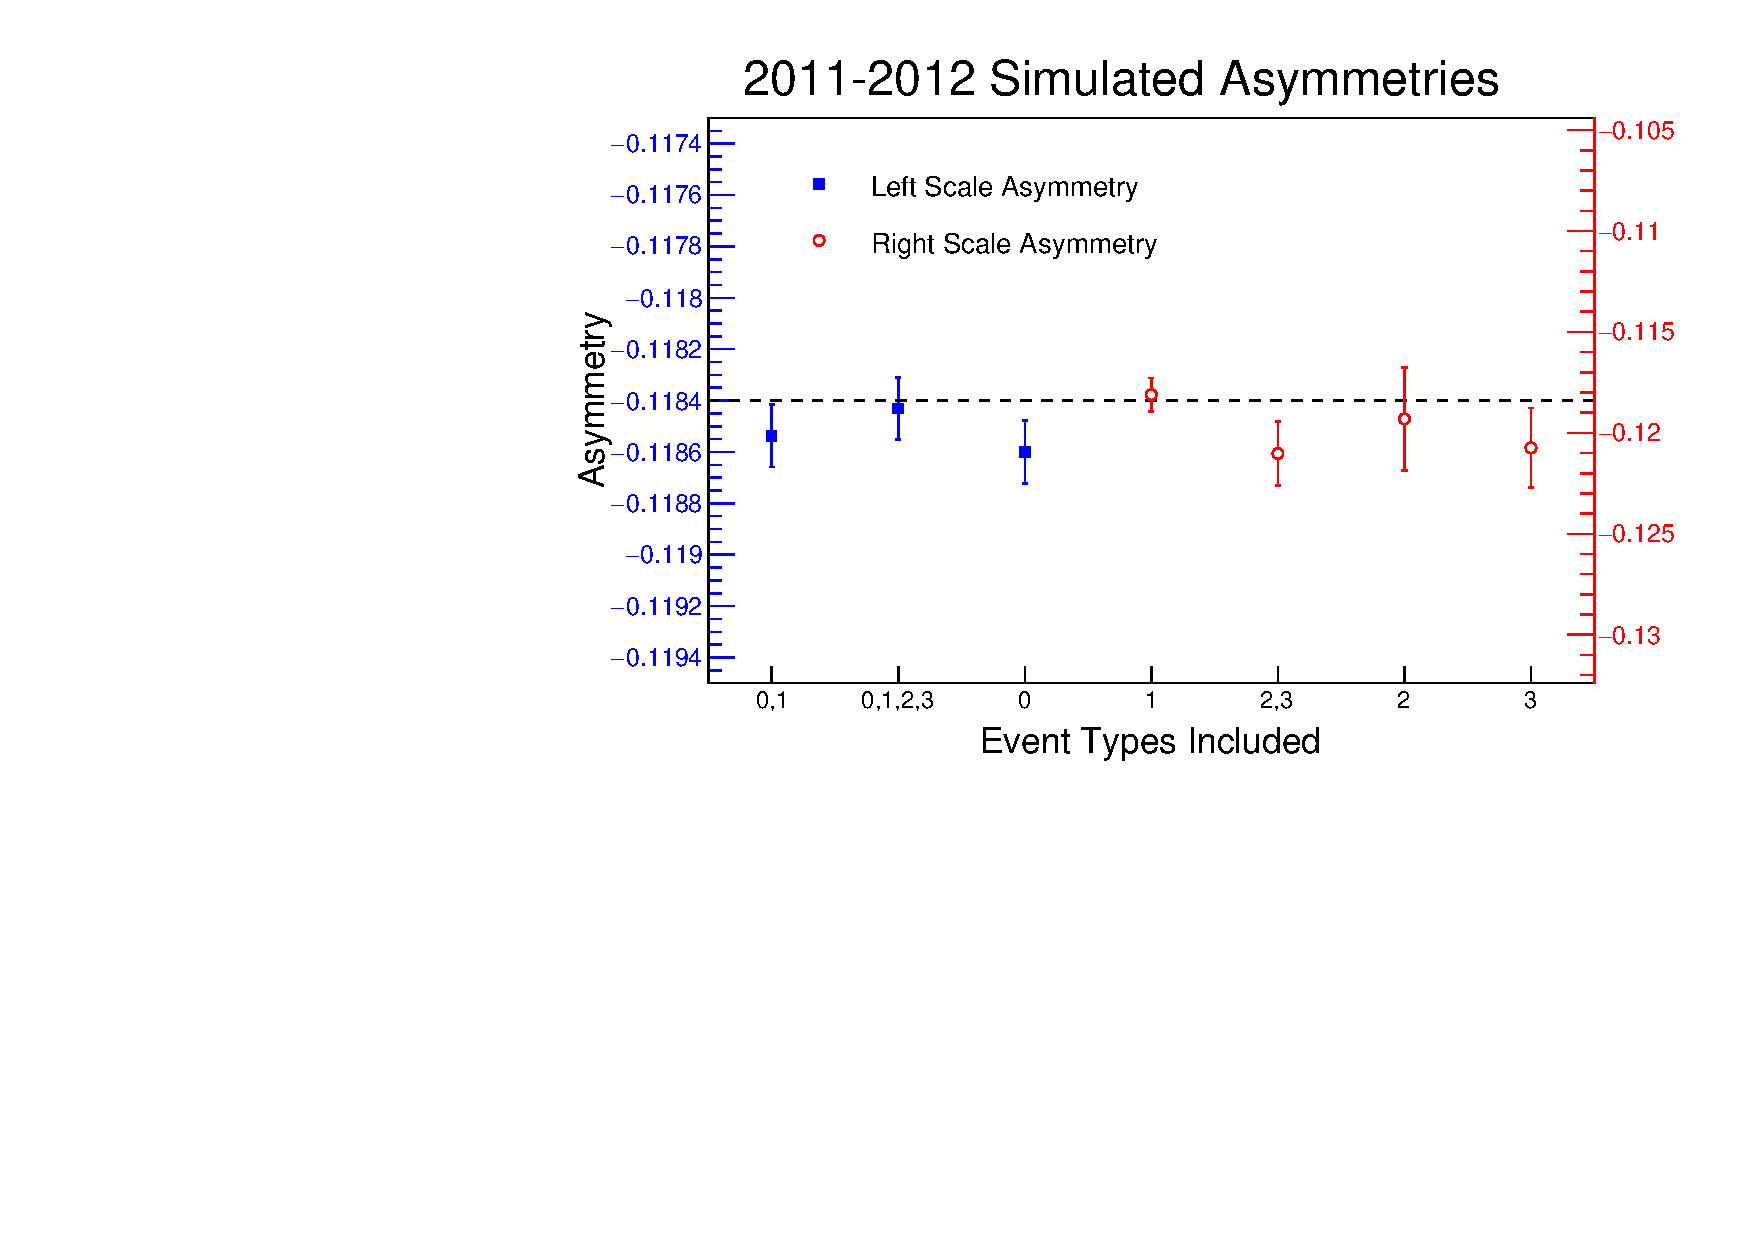
\includegraphics[page=1,scale=0.5]{5-UCNAResults/asymms_doubleAxis_AllCorr__color.pdf}} \\ 
    \subfloat[2012-2013]{\includegraphics[page=2,scale=0.5]{5-UCNAResults/asymms_doubleAxis_AllCorr__color.pdf}}
  \end{tabular}
  \caption{Extracted asymmetries from Monte Carlo data processed to mimic the
    experimental data. The dashed line indicates the 2017 PDG value $A_0 = -0.1184$
    which was input into the simulation, thus the goal upon extraction of the final
    asymmetry parameter. The blue closed points indicate analysis choices that include
    type 0 events and utilize the scale on the left vertical axis values. The red open circles
    include only backscattering event types and use the right vertical axis values.}
  \label{fig:MCasymm}
\end{figure}


\subsection{Polarimetry Correction} \label{ssec:polCorr}

As mentioned in Section \ref{sec:polarimetry}, an equilibrium population of neutron
spins develops within the decay trap during a $\beta$-decay run. While this population is
dominated by the spin-state of choice ($>99\%$), precise determination of the average
polarization is important as it directly affects the final extracted asymmetry as shown in
equation \ref{eq:A0}. The determination of the polarization values was carried
out in a separate analysis by Eric Dees of North Carolina State University.
The values for the $\pm$ spin-flipper states for
each geometry are given in table \ref{tab:pol}.

\setlength{\tabcolsep}{12pt}
\begin{table}[h]
  \caption{Results for average polarization fractions for each dataset in spin-flipper off ($-$)
    and spin-flipper on ($+$) states.} 
  \centering
  \begin{tabular}{c c c c}
    \hline \hline \\ [-1.75ex]
    \multicolumn{2}{c}{2011-2012}&\multicolumn{2}{c}{2012-2013} \\ [0.5ex]
    $\langle P \rangle_-$ & $\langle P \rangle_+$ & $\langle P \rangle_-$ & $\langle P\rangle_+$ \\ [0.25ex]
    \hline \\ [-1.75ex]
    %$\Delta P/P$ (\%) & 0.30 & 0.25 & 0.15 & 0.20 \\ [0.25ex]
    0.9970(30) & 0.9939(25) & 0.9979(15) & 0.9952(20) \\ [0.25ex]
    \hline
  \end{tabular}
  \label{tab:pol}
\end{table}

There are two options for applying a polarization correction, namely
calculate an average polarization $\langle P \rangle$
which is averaged over both spin states and simply
divide this out of the measured asymmetry as shown in Equation \ref{eq:A0}, or utilize the
separate $\langle P\rangle_\pm$ values. The second method is not a simple division of
either term but rather a more complicated combination due to the usage of the super-ratio.
This second method was adopted for this analysis and is described below.

\subsubsection{Extraction of $A_0$ Using $\langle P \rangle_+$ and $\langle P \rangle_-$}
\label{ssec:polSep}

Using each of the $\langle P\rangle_\pm$ values requires modification of our initial
asymmetry formalism from \ref{sec:asymmetry} \cite{ARYoungPol}. We can no longer make
the assumption that $\langle P\rangle_+ = \langle P\rangle_-$ if we want to treat them
separately. Let us start our new derivation from Equation \ref{eq:decayRate}, which now
becomes
%
\begin{equation} \label{eq:POLdecayRate}
  \Gamma_{1,2}^{\pm}\left(E\right)=C' \cdot S(E) \cdot \epsilon_{\pm} \cdot \eta_{1,2}
  \left[ 1 \pm_{1,2} 
    \left(\mp \langle P \rangle_\pm \right) \cdot A(E) \frac{\beta}{2} \right]
\end{equation}
%
\noindent under the substition $\langle P\rangle \rightarrow \langle P\rangle_\pm$.

The super-ratio now must be written as
%
\begin{equation*}
  R = \frac{\Gamma_{1}^+ \cdot \Gamma_{2}^-}{\Gamma_{1}^- \cdot \Gamma_{2}^+} 
  =  \frac{ \left[ 1 + \left(- \langle P \rangle_+ \right)  A(E) \frac{\beta}{2} \right] 
\left[ 1 - \left(+ \langle P \rangle_- \right)  A(E) \frac{\beta}{2} \right]  }
{  \left[ 1 +  \left(+ \langle P \rangle_- \right)  A(E) \frac{\beta}{2}  \right] 
 \left[ 1 -  \left(- \langle P \rangle_+ \right)  A(E) \frac{\beta}{2} \right]},
\end{equation*}
%
\noindent and upon letting $\xi = A(E)\frac{\beta}{2}$ we have
%
\begin{equation} \label{eq:polR}
  R =  \frac{ \Big( 1 - \xi \langle P \rangle_+ \Big)
    \Big( 1 - \xi \langle P \rangle_- \Big) }
{  \Big( 1 + \xi \langle P \rangle_- \Big)
    \Big( 1 + \xi \langle P \rangle_+ \Big) }.
\end{equation}

We are interested in solving for $A(E)$, or $\xi$, so we can rearrange \ref{eq:polR} to give
%
\begin{equation*}
  R\Big( 1 + \xi \langle P \rangle_- \Big) \Big( 1 + \xi \langle P \rangle_+ \Big) =
  \Big( 1 - \xi \langle P \rangle_+ \Big)
    \Big( 1 - \xi \langle P \rangle_- \Big),
\end{equation*}
%
\begin{equation*}
  R\bigg( 1 + \xi \Big(\langle P \rangle_-+\langle P \rangle_+ \Big) + \xi^2\langle P \rangle_-
  \langle P \rangle_+\bigg) =
  \bigg( 1 - \xi \Big(\langle P \rangle_-+\langle P \rangle_+ \Big) + \xi^2\langle P \rangle_-
  \langle P \rangle_+\bigg),
\end{equation*}
%
\begin{equation*}
  0 = \xi^2\langle P \rangle_- \langle P \rangle_+\Big(1-R\Big)
  - \xi\Big(\langle P \rangle_-+\langle P \rangle_+ \Big)\Big(1+R\Big)
  + \Big(1-R\Big),
\end{equation*}
%
\noindent and
%
\begin{equation}
  0 = \xi^2\langle P \rangle_- \langle P \rangle_+
  - \xi\Big(\langle P \rangle_-+\langle P \rangle_+ \Big)\bigg(\frac{1+R}{1-R}\bigg)
  + 1,
\end{equation}
%
\noindent which has roots (let $\gamma = \frac{1+R}{1-R}$)
%
\begin{equation}
  \xi = \frac{\gamma\Big(\langle P \rangle_-+\langle P \rangle_+ \Big)
    \pm \sqrt{\gamma^2\Big(\langle P \rangle_-+\langle P \rangle_+ \Big)^2
      -4\langle P \rangle_- \langle P \rangle_+}}
      {2\langle P \rangle_- \langle P \rangle_+}.
\end{equation}

To choose the proper root, we set
$\langle P \rangle_- = \langle P \rangle_+ = \langle P \rangle$ and determine
which root returns the original expression for the super-ratio as given in equations
\ref{eq:A_SR_frac} and \ref{eq:A_SR}, namely
%
\begin{equation*} \label{eq:A_SR}
  A_{\mathrm{SR}} = \frac{1-\sqrt{R}}{1+\sqrt{R}} = \langle P
  \rangle  A(E)  \frac{\beta}{2}.
\end{equation*}
%
\noindent Upon doing so, we find that the negative root is the correct
solution, which results in a new expression for $A(E)$ of
%
\begin{equation}
  A(E) = \frac{\gamma\Big(\langle P \rangle_-+\langle P \rangle_+ \Big)
    - \sqrt{\gamma^2\Big(\langle P \rangle_-+\langle P \rangle_+ \Big)^2
      -4\langle P \rangle_- \langle P \rangle_+}}
      {\beta\langle P \rangle_- \langle P \rangle_+}.
\end{equation}

The uncertainty on $A(E)$ from such an application of the polarization is determined via
the usual error propagation,
%
\begin{equation}
  \delta_PA(E) = \sqrt{\bigg(\frac{\partial A(E)}{\partial \langle P \rangle_+}\bigg)^2
    \Big(\delta \langle P \rangle_+\Big)^2 +
    \bigg( \frac{\partial A(E)}{\partial \langle P \rangle_-}\bigg)^2
    \Big(\delta \langle P \rangle_-\Big)^2}.
\end{equation}
%
Although this method of determining the measured asymmetry is more rigorous than using a
polarimetry value averaged over the two spin states, the effect on the asymmetry is
at the $\Delta A \approx 10^{-6}$ level as shown by K. Hickerson in \cite{hickerson2013}.
A change in the asymmetry of this magnitude is small compared to the uncertainty from
the polarization alone and inconsequential compared
to the final uncertainty on the asymmetry. 


\subsection{Energy Reconstruction} \label{ssec:energyRecon}

The energy enters the calculation of the asymmetry in the $\beta$ term ($v/c$ of the
electron) in Equation \ref{eq:A_SR}, and thus it is essential to assess how well
we can reconstruct the initial energy of an electron. The obvious choice for determining
the efficacy of our energy calibration is to use the calibration peaks themselves and
compare to Monte Carlo simulation. We apply the calibrations from
Chapter \ref{ch:UCNA_Calibrations} to the data source peaks in all
individual source runs,
which maps the detector response to a reconstructed peak energy ($E_{\mathrm{recon}}^{\mathrm{data}}$),
and then we apply our
detector response model to the simulation peaks and extract a Monte Carlo reconstructed peak energy
($E_{\mathrm{recon}}^{\mathrm{MC}}$). We can then calculate a residual for every single run (and each
conversion peak within that run) via
$\mathrm{Residual} = E_{\mathrm{recon}}^{\mathrm{data}} - E_{\mathrm{recon}}^{\mathrm{MC}}$. Upon collecting all
of the residuals for each of the conversion electron peaks (Figures \ref{fig:residuals2011}
and \ref{fig:residuals2012}), we calculate
\footnote{ \label{fn:sourceMean}The mean and sigma are calculated rather than fitted so as to not neglect any
  non-Gaussian tails in the distributions.} the mean and sigma of the distributions, with
values reported in table \ref{tab:residuals}, and use
them as the data points seen in Figure \ref{fig:errEnv}. These points are a measure
of the accuracy of the energy calibration at four discrete energies, the mean energies of the
conversion electron lines themselves.

\begin{figure}[h]
  \centering
  \begin{tabular} {c c}
    \subfloat[$^{137}\mathrm{Ce}$ Conversion Line]{\includegraphics[page=11,scale=0.35]{5-UCNAResults/final_residuals_1-12.pdf}} &
    \subfloat[$^{113}\mathrm{Sn}$ Conversion Line]{\includegraphics[page=13,scale=0.35]{5-UCNAResults/final_residuals_1-12.pdf}} \\
    \subfloat[Lower $^{207}\mathrm{Bi}$ Conversion Line]{\includegraphics[page=14,scale=0.35]{5-UCNAResults/final_residuals_1-12.pdf}} &
    \subfloat[Upper $^{207}\mathrm{Bi}$ Conversion Line]{\includegraphics[page=15,scale=0.35]{5-UCNAResults/final_residuals_1-12.pdf}}
  \end{tabular}
  \caption{Distributions of the residuals for each conversion electron source line used in the 2011-2012 calibration.
    The mean and sigma reported in the fit box are not the same as those used in the energy uncertainty, as they
    are the results of the fit and not the calculated mean.}
  \label{fig:residuals2011}
\end{figure}

\begin{figure}[h]
  \centering
  \begin{tabular} {c c}
    \subfloat[$^{137}\mathrm{Ce}$ Conversion Line]{\includegraphics[page=11,scale=0.35]{5-UCNAResults/final_residuals_16-24.pdf}} &
    \subfloat[$^{113}\mathrm{Sn}$ Conversion Line]{\includegraphics[page=13,scale=0.35]{5-UCNAResults/final_residuals_16-24.pdf}} \\
    \subfloat[Lower $^{207}\mathrm{Bi}$ Conversion Line]{\includegraphics[page=14,scale=0.35]{5-UCNAResults/final_residuals_16-24.pdf}} &
    \subfloat[Upper $^{207}\mathrm{Bi}$ Conversion Line]{\includegraphics[page=15,scale=0.35]{5-UCNAResults/final_residuals_16-24.pdf}}
  \end{tabular}
  \caption{Distributions of the residuals for each conversion electron source line used in the 2012-2013 calibration.
    The mean and sigma reported in the fit box are not the same as those used in the energy uncertainty, as they
    are the results of the fit and not the calculated mean.}
  \label{fig:residuals2012}
\end{figure}

%\setlength{\tabcolsep}{12pt}
\begin{table}[h]
  \caption{Mean and $\sigma$ of each conversion electron residual distribution
  as used in the energy uncertainty, Figure \ref{fig:errEnv}.} 
  \centering
  \begin{tabular}{c c c}
    \hline \hline \\ [-1.75ex]
    & 2011-2012 & 2011-2012 \\
    \hline \\ [-1.75ex]
    $^{137}\mathrm{Ce}$ & $-1.43\pm1.81$~keV & $-0.80\pm2.00$~keV \\
    $^{113}\mathrm{Sn}$ & $0.91\pm2.52$~keV & $-2.24\pm2.87$~keV \\
    $^{207}\mathrm{Bi}$ (lower) & $-1.36\pm3.81$~keV & $-0.39\pm3.90$~keV \\
    $^{207}\mathrm{Bi}$ (upper) & $-1.55\pm5.77$~keV & $0.01\pm6.40$~keV \\
    \hline
  \end{tabular}
  \label{tab:residuals}
\end{table}

\begin{figure}[h]
\centering
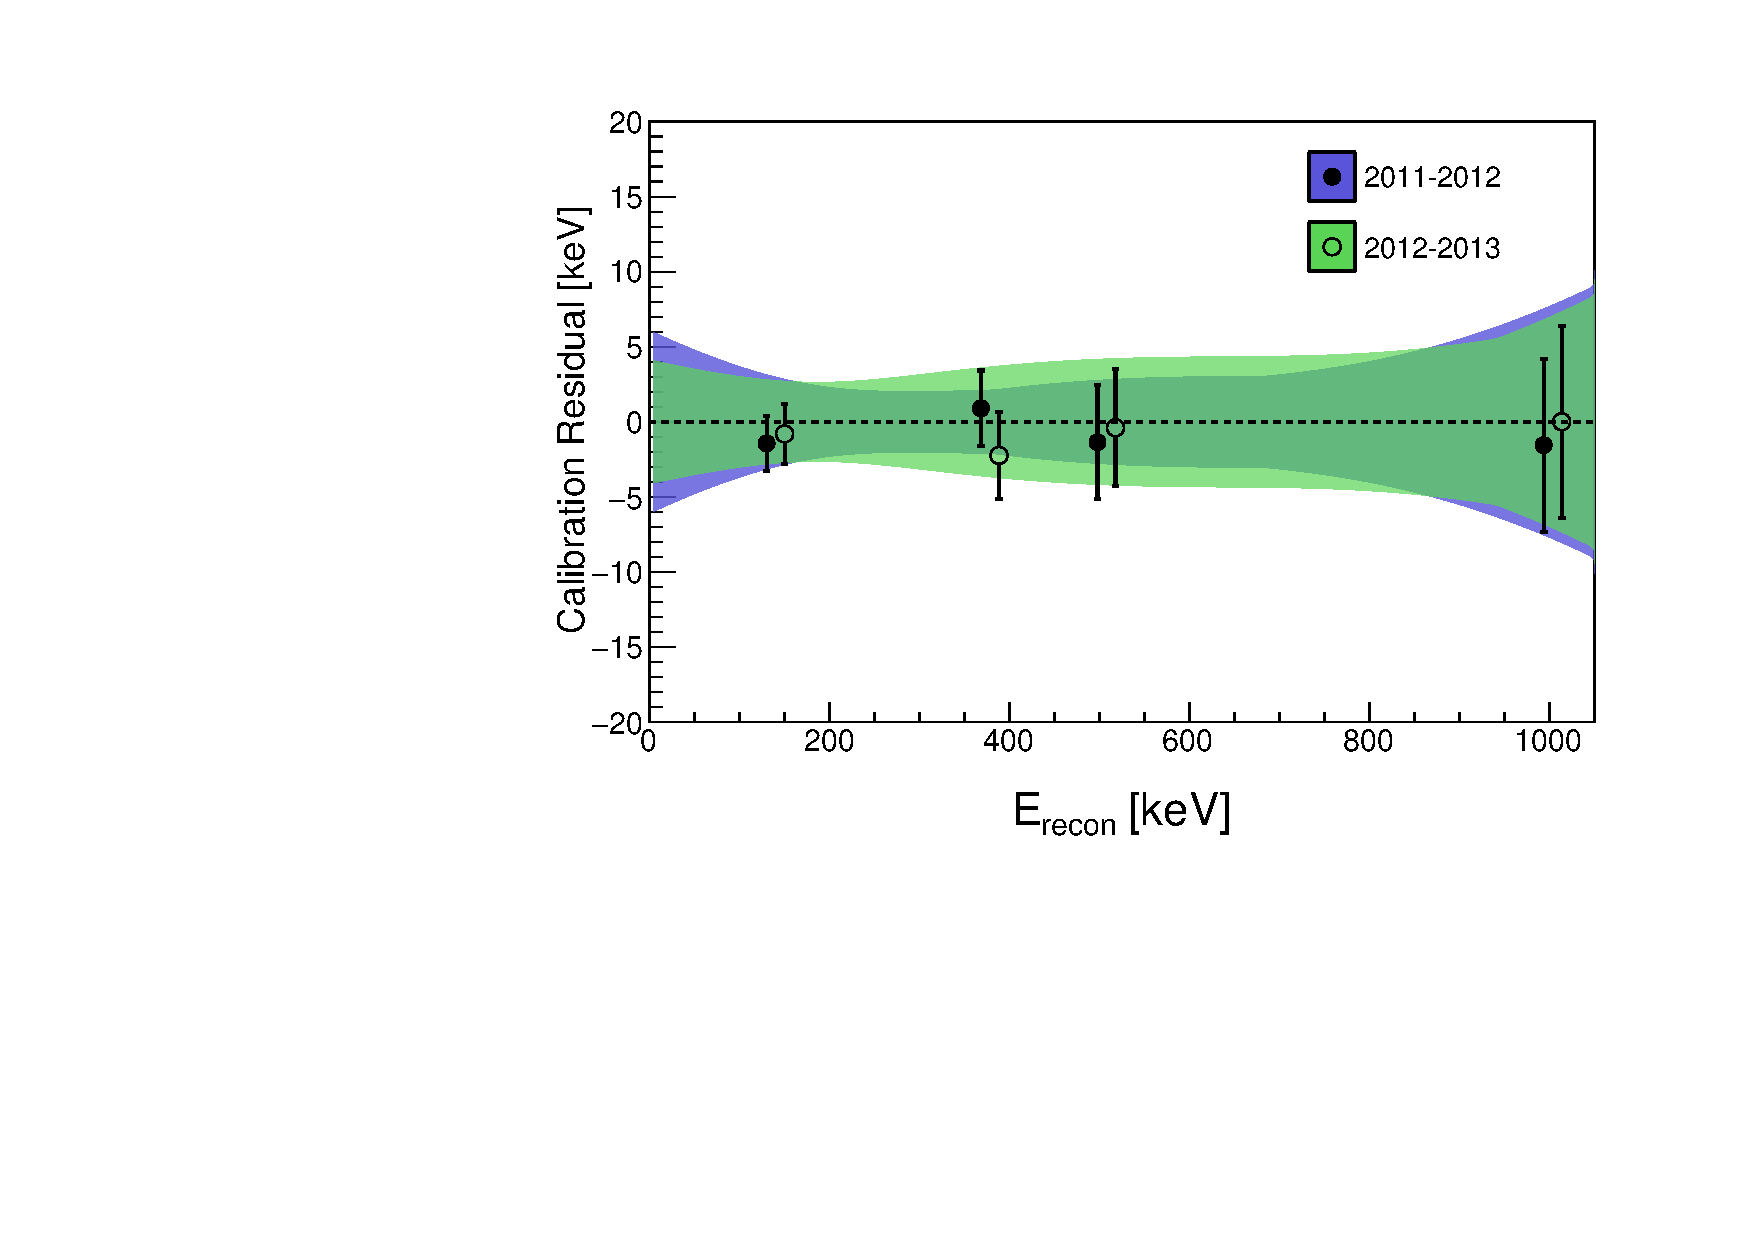
\includegraphics[scale=.65]{5-UCNAResults/energyErrorEnvelope_color.pdf}
\caption{Plot of energy uncertainty vs. reconstructed energy. The points plotted are the mean
  and $\sigma$ of all reconstructed calibration peaks of $^{137}\mathrm{Ce}$,
  $^{113}\mathrm{Sn}$, and the lower and
  upper $^{207}\mathrm{Bi}$ peaks in that order. The $x$-axis offset in the 2011-2012 and 2012-2013 points is
  artificial and only meant for visualization. The bands represent the energy uncertainty
  at any given electron energy for the two data sets.}
\label{fig:errEnv}
\end{figure}

\begin{figure}[h]
\centering
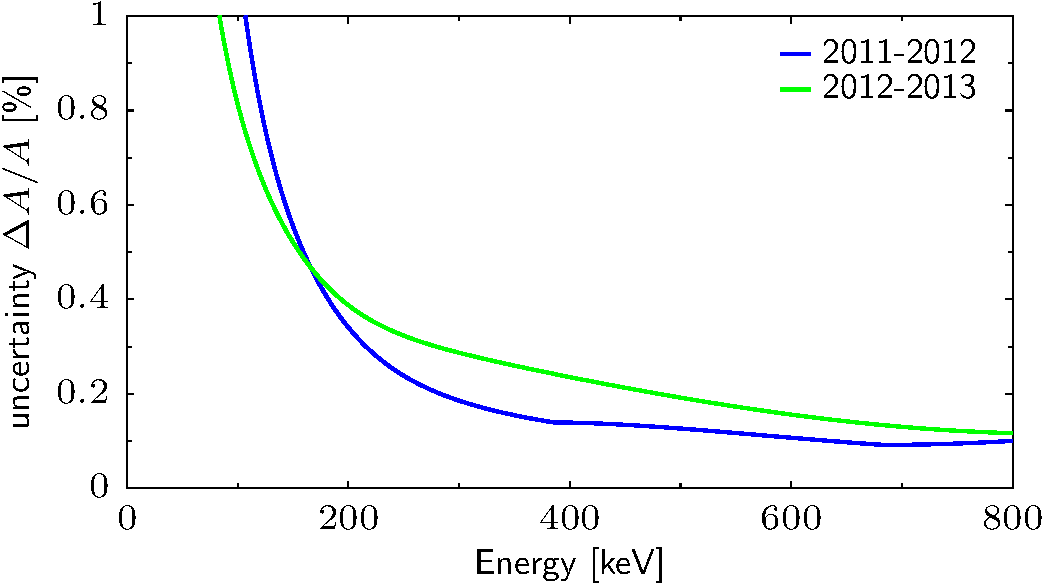
\includegraphics[scale=.50]{5-UCNAResults/EnergyUncertALL.pdf}
\caption{Plot of uncertainty on $A_0$ from the energy calibration vs. reconstructed energy
  for each of the 2011-2012 and 2012-2013 geometries. Weighting the energy dependent
  uncertainties shown here by the experimental statistics in each energy bin produces
  the final uncertainty on the extracted asymmetries.}
\label{fig:energyUncert}
\end{figure}

The residuals at these discrete energies do not
themselves tell us how well we do at intermediate energies. In the past, a conservative
uncertainty envelope was drawn to encompass the calibration points
\cite{mendenhall2013,mpmThesis}. For the analysis
presented here, a more quantitative determination of the uncertainty envelope was employed
via methods developed by K. Hickerson for determination of limits on $b_n$ from the previous
UCNA spectrum (\cite{hickerson2017}). In short, the envelope is produced by sampling
the coefficients of a quadratic, $f(E_{\mathrm{recon}})$, from distributions that reproduce
the residual data points seen in Figure \ref{fig:errEnv} with $1\sigma$ deviation.
This
obviously results in an asymmetric uncertainty band due to the asymmetric distribution
of the data points about zero, but our conservative approach is
to take the worst case uncertainty at every energy and use this as our
symmetric final uncertainty.
This produces the symmetric uncertainty band in Figure \ref{fig:errEnv}.

The symmetric worst case uncertainty band allows us to report a systematic uncertainty
rather than a correction and an uncertainty from the energy reconstruction. The energy
dependent uncertainty on $A_0$ for the maximal energy uncertainty (outer edge of the
uncertainty envelope) is shown in Figure \ref{fig:energyUncert}.
The uncertainty is then weighted by the data statistics in each bin to determine the
total uncertainty in the final asymmetry, producing energy uncertainties of $0.17\%$ and
$0.25\%$ for 2011-2012 and 2012-2013 respectively.

\subsection{Background Contributions}

The desired events (foreground) are superposed with background
triggering events from something other
than a neutron $\beta$-decay within the decay trap. Such unwanted events include
background ambient
gamma rays, cosmic rays,
and other unforeseen events which trigger the detector.
Gamma ray events are highly suppressed due to the
requirement of a coincidence trigger between the MWPC and the scintillator,
and cosmic ray muon events are removed using a series of muon veto
detection packages, which leaves the rest of the background to be subtracted using direct
measurements of the electron spectrum in the absence of neutrons in the decay trap.

\subsubsection{Background Subtraction} \label{sssec:bgsubtr}

Accompanying every $\beta$-decay run is a dedicated background run roughly $1/4$ the
length of the data taking run. The background events are processed in an identical manner
to the data events and the rates are subtracted from the data rates. The uncertainties are
propagated into the final rate, so in the absence of any non-statistical background
fluctuations, the uncertainties from the backgrounds are inherently included in the extraction
of the asymmetry. The background spectra for the different event types can be seen in figures
\ref{fig:bgSpectra2011} and \ref{fig:bgSpectra2012}.
%
\begin{figure}[h]
  \centering
  \begin{tabular} {c c}
    \subfloat[Type 0]{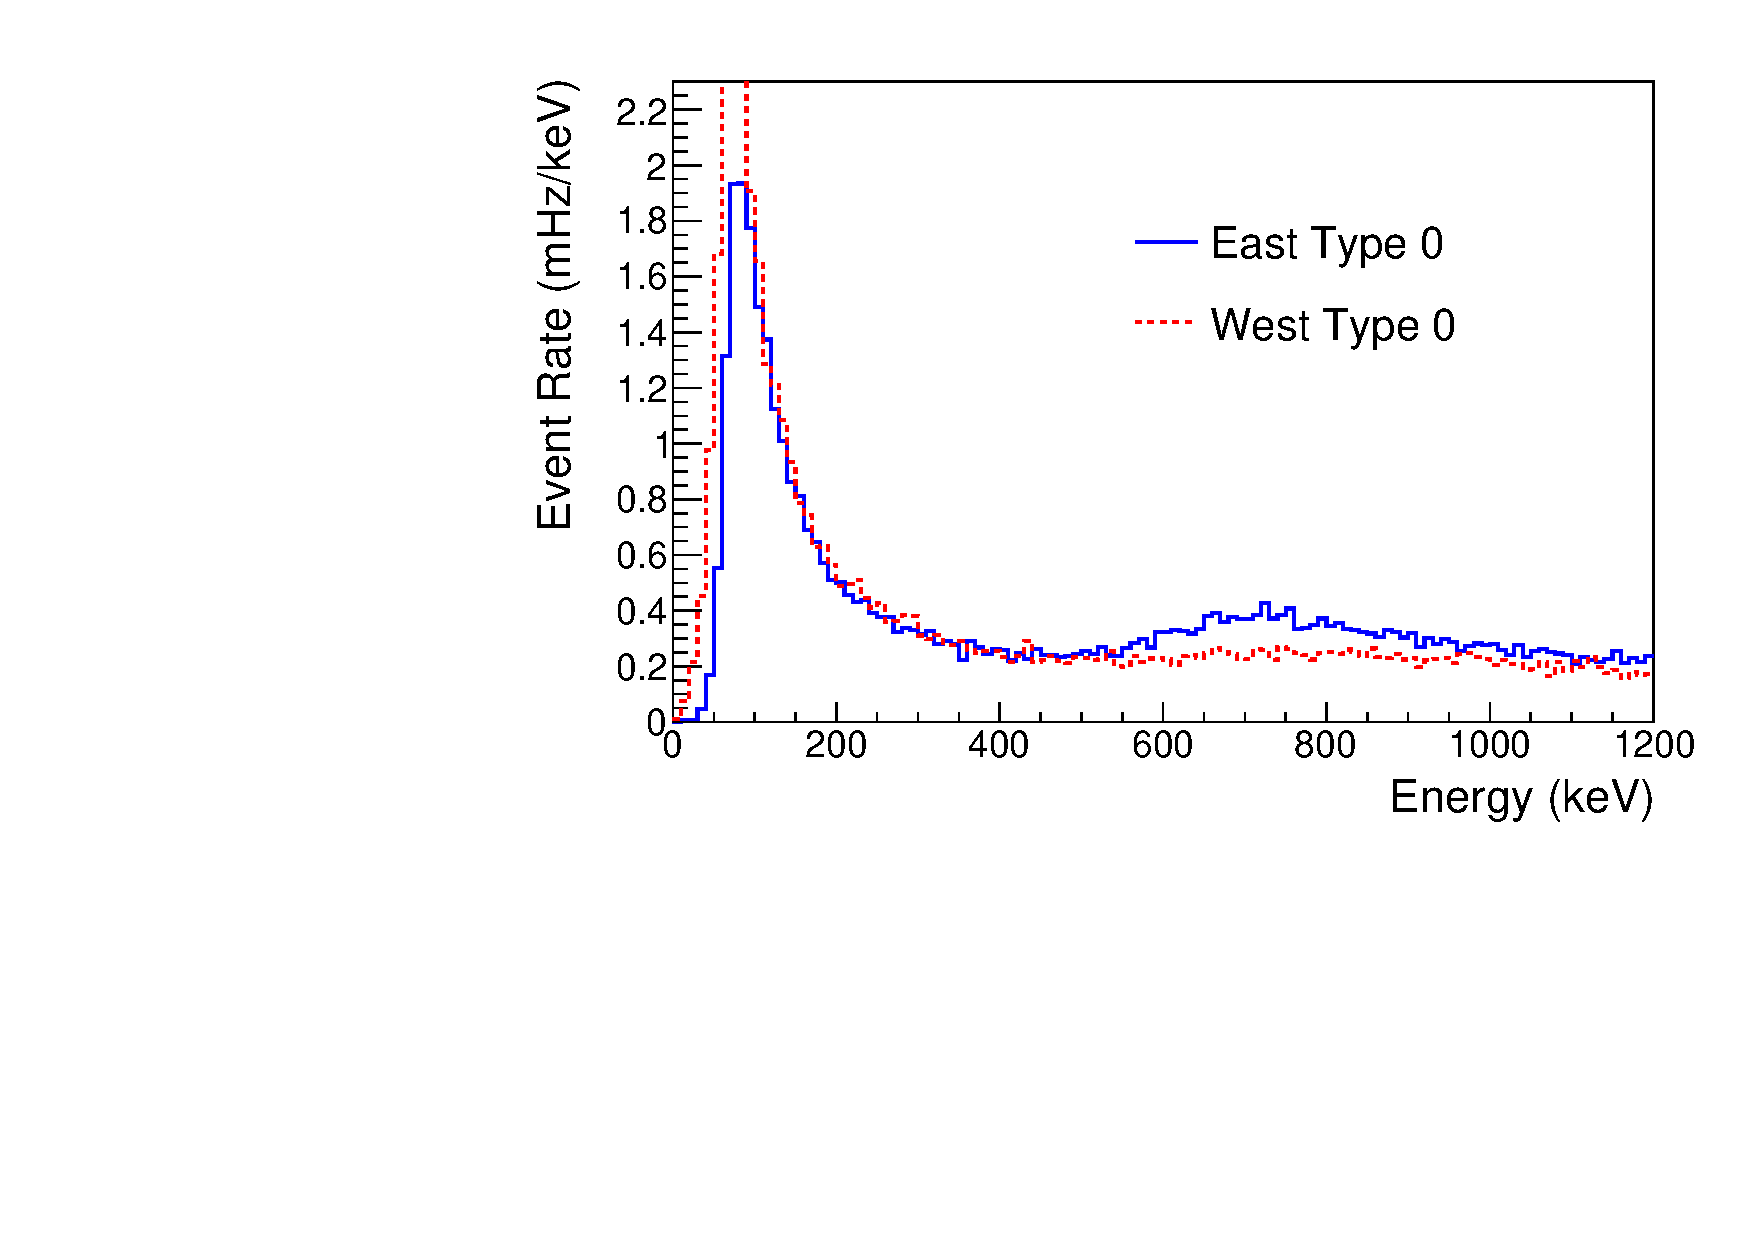
\includegraphics[page=1,scale=0.30]{5-UCNAResults/bgSpectra_octets0-59.pdf}} &
    \subfloat[Type 1]{\includegraphics[page=2,scale=0.30]{5-UCNAResults/bgSpectra_octets0-59.pdf}} \\
    \subfloat[Type 2]{\includegraphics[page=3,scale=0.30]{5-UCNAResults/bgSpectra_octets0-59.pdf}} &
    \subfloat[Type 3]{\includegraphics[page=4,scale=0.30]{5-UCNAResults/bgSpectra_octets0-59.pdf}}
  \end{tabular}
  \caption{Total background spectra summed over all background runs for each event type in
   2011-2012.}
  \label{fig:bgSpectra2011}
\end{figure}
\begin{figure}[h]
  \centering
  \begin{tabular} {c c}
    \subfloat[Type 0]{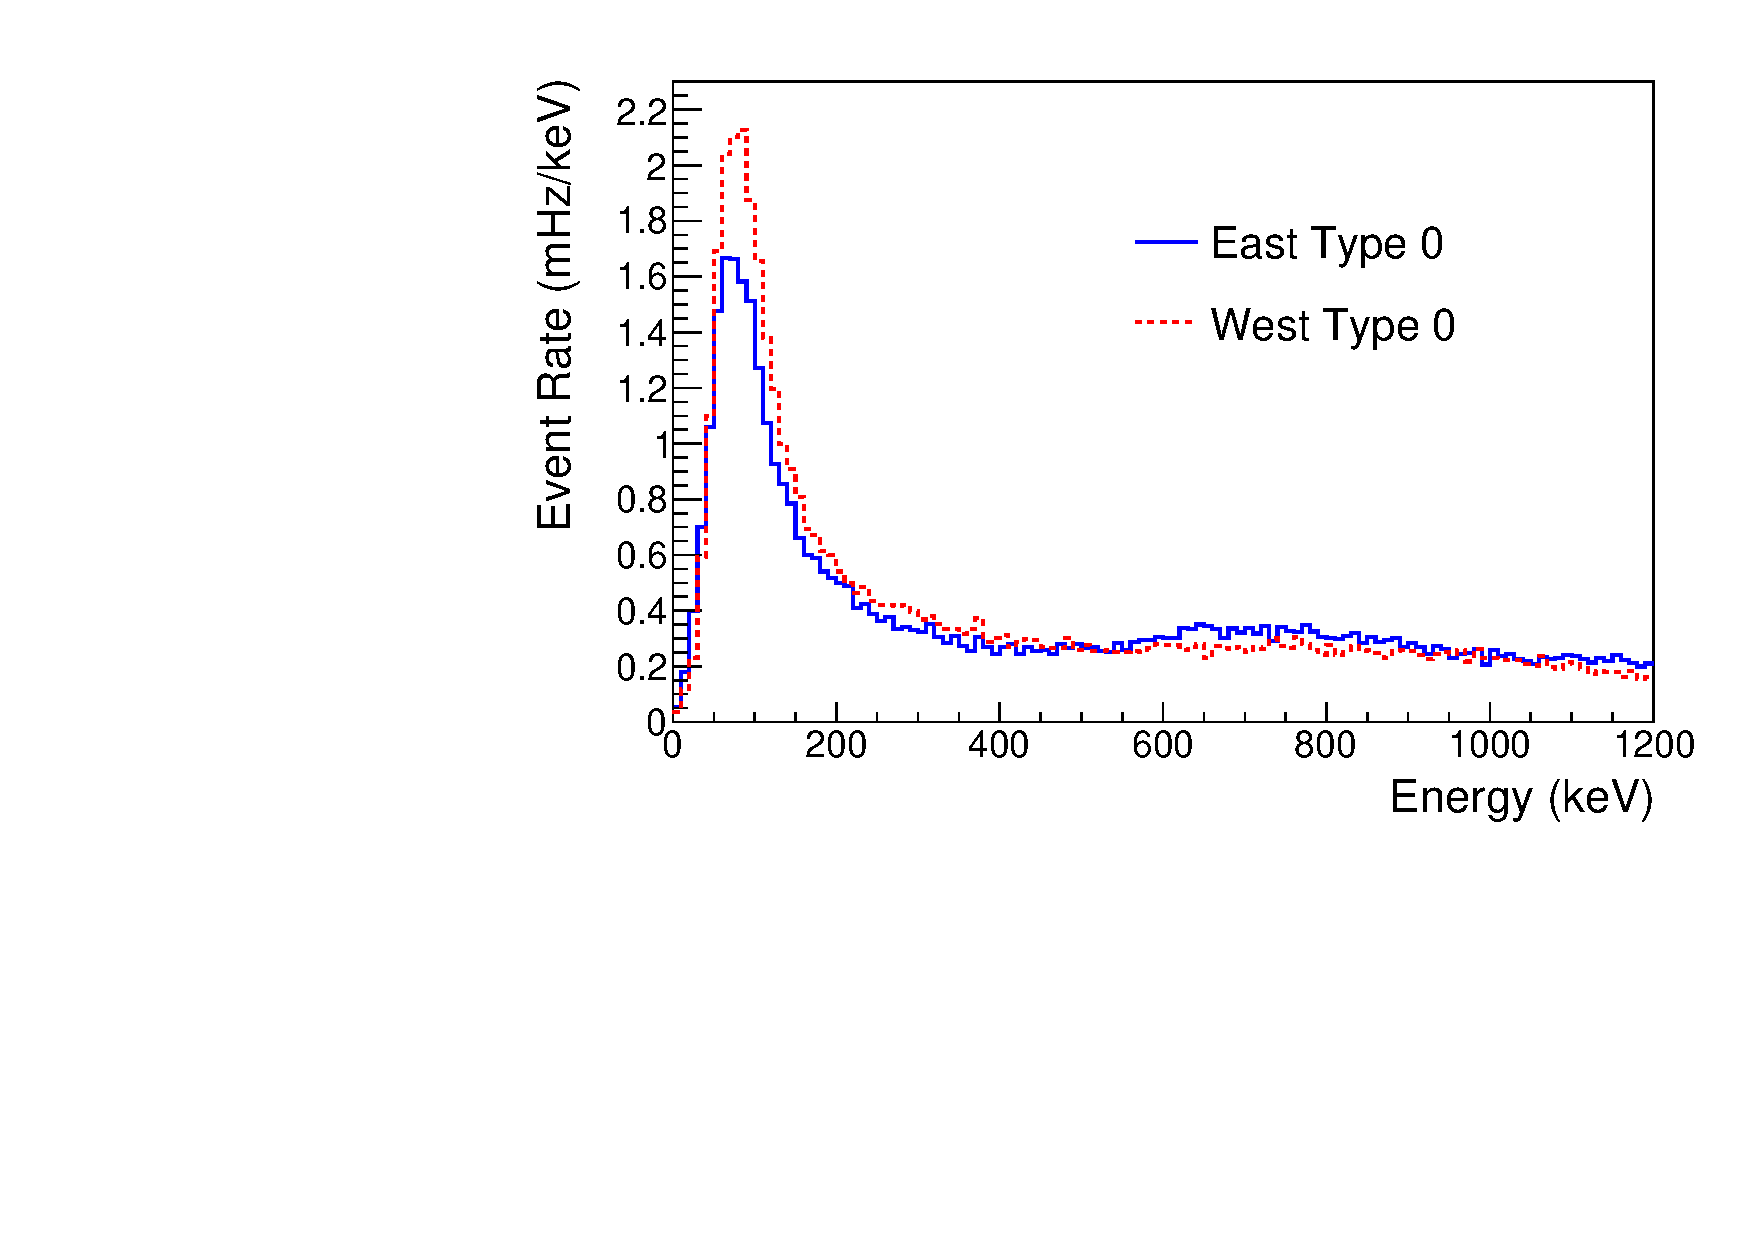
\includegraphics[page=1,scale=0.30]{5-UCNAResults/bgSpectra_octets60-121.pdf}} &
    \subfloat[Type 1]{\includegraphics[page=2,scale=0.30]{5-UCNAResults/bgSpectra_octets60-121.pdf}} \\
    \subfloat[Type 2]{\includegraphics[page=3,scale=0.30]{5-UCNAResults/bgSpectra_octets60-121.pdf}} &
    \subfloat[Type 3]{\includegraphics[page=4,scale=0.30]{5-UCNAResults/bgSpectra_octets60-121.pdf}}
  \end{tabular}
  \caption{Total background spectra summed over all background runs for each event type in
   2011-2012.}
  \label{fig:bgSpectra2012}
\end{figure}

The typical ratio between data and background rates is roughly 70:1 in 2011-2012 and
40:1 in 2012-2013 when integrated over the electron energy range 190-740~keV,
with the difference attributed to source performance issues. Figures
\ref{fig:integratedRates2011} and \ref{fig:integratedRates2012} show the integrated
rates in $\beta$-decay runs and background runs for the two geometries. The splitting in the
$\beta$ run rates is due to the difference between a spin-flipper ``on'' vs. spin-flipper
``off'' run, as the flipper ``on'' loading efficiency is $\sim 2/3$ that of
a flipper ``off'' run. This difference results from electrons being boosted by roughly 120~neV
from the change in potential
associated with a spin flip in the $\sim 1$~T field in the AFP spin-flipper, which moves a
portion of the neutrons out of the UCN energy regime and thus they are no longer confined
within the decay trap.

%
\begin{figure}[h]
  \centering
  \begin{tabular} {cc}
    \subfloat[East Side]{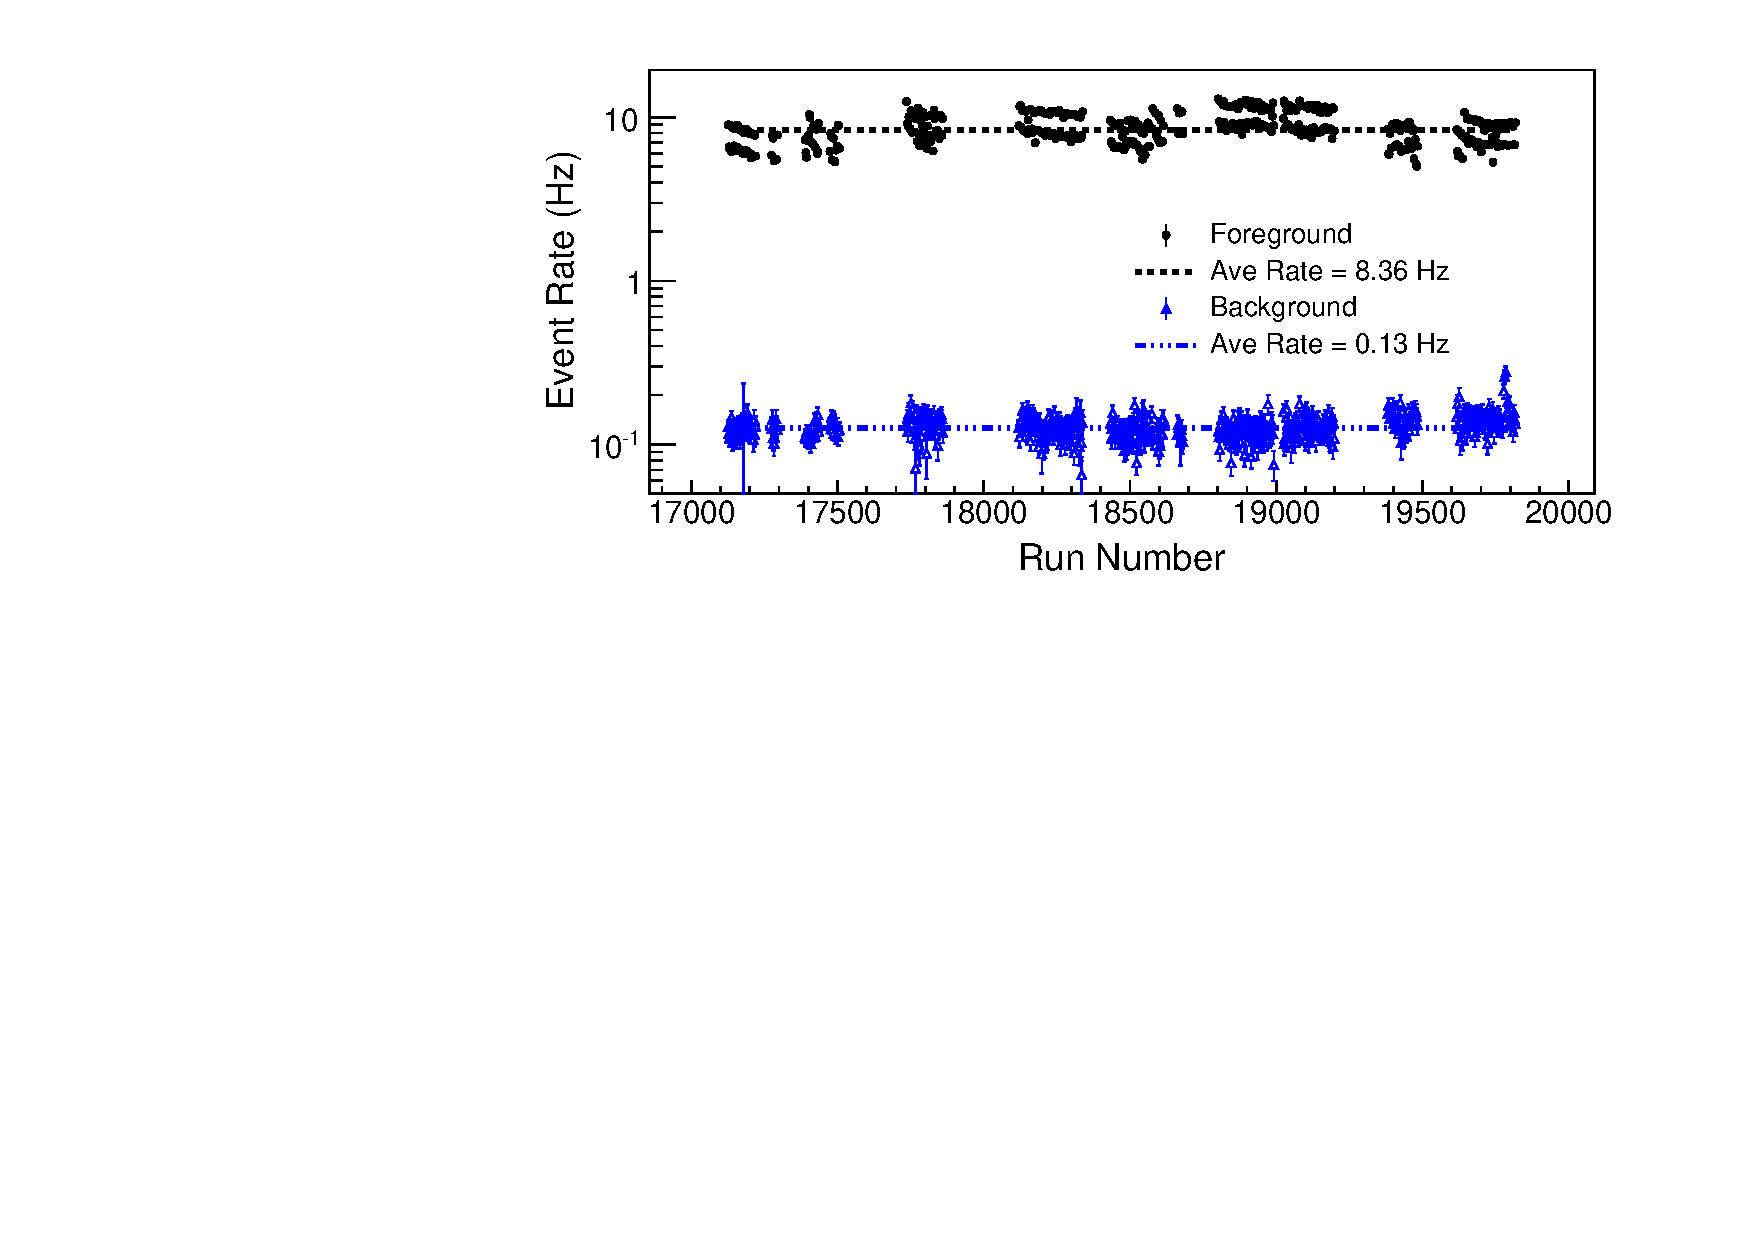
\includegraphics[page=1,scale=0.5]{5-UCNAResults/integratedRatesByRun_2011-2012_anaChC_190-740.pdf}} \\
    \subfloat[West Side]{\includegraphics[page=2,scale=0.5]{5-UCNAResults/integratedRatesByRun_2011-2012_anaChC_190-740.pdf}}     
  \end{tabular}
  \caption{Integrated event rates for 2011-2012 East and West sides. The splitting in the
$\beta$ run rates is due to the difference between a spin-flipper ``on'' vs. spin-flipper
``off'' run, as the flipper ``on'' loading efficiency is approximately 2/3 that of
a flipper ``off'' run.}
  \label{fig:integratedRates2011}
\end{figure}
\begin{figure}[h]
  \centering
  \begin{tabular} {c}
    \subfloat[East Side]{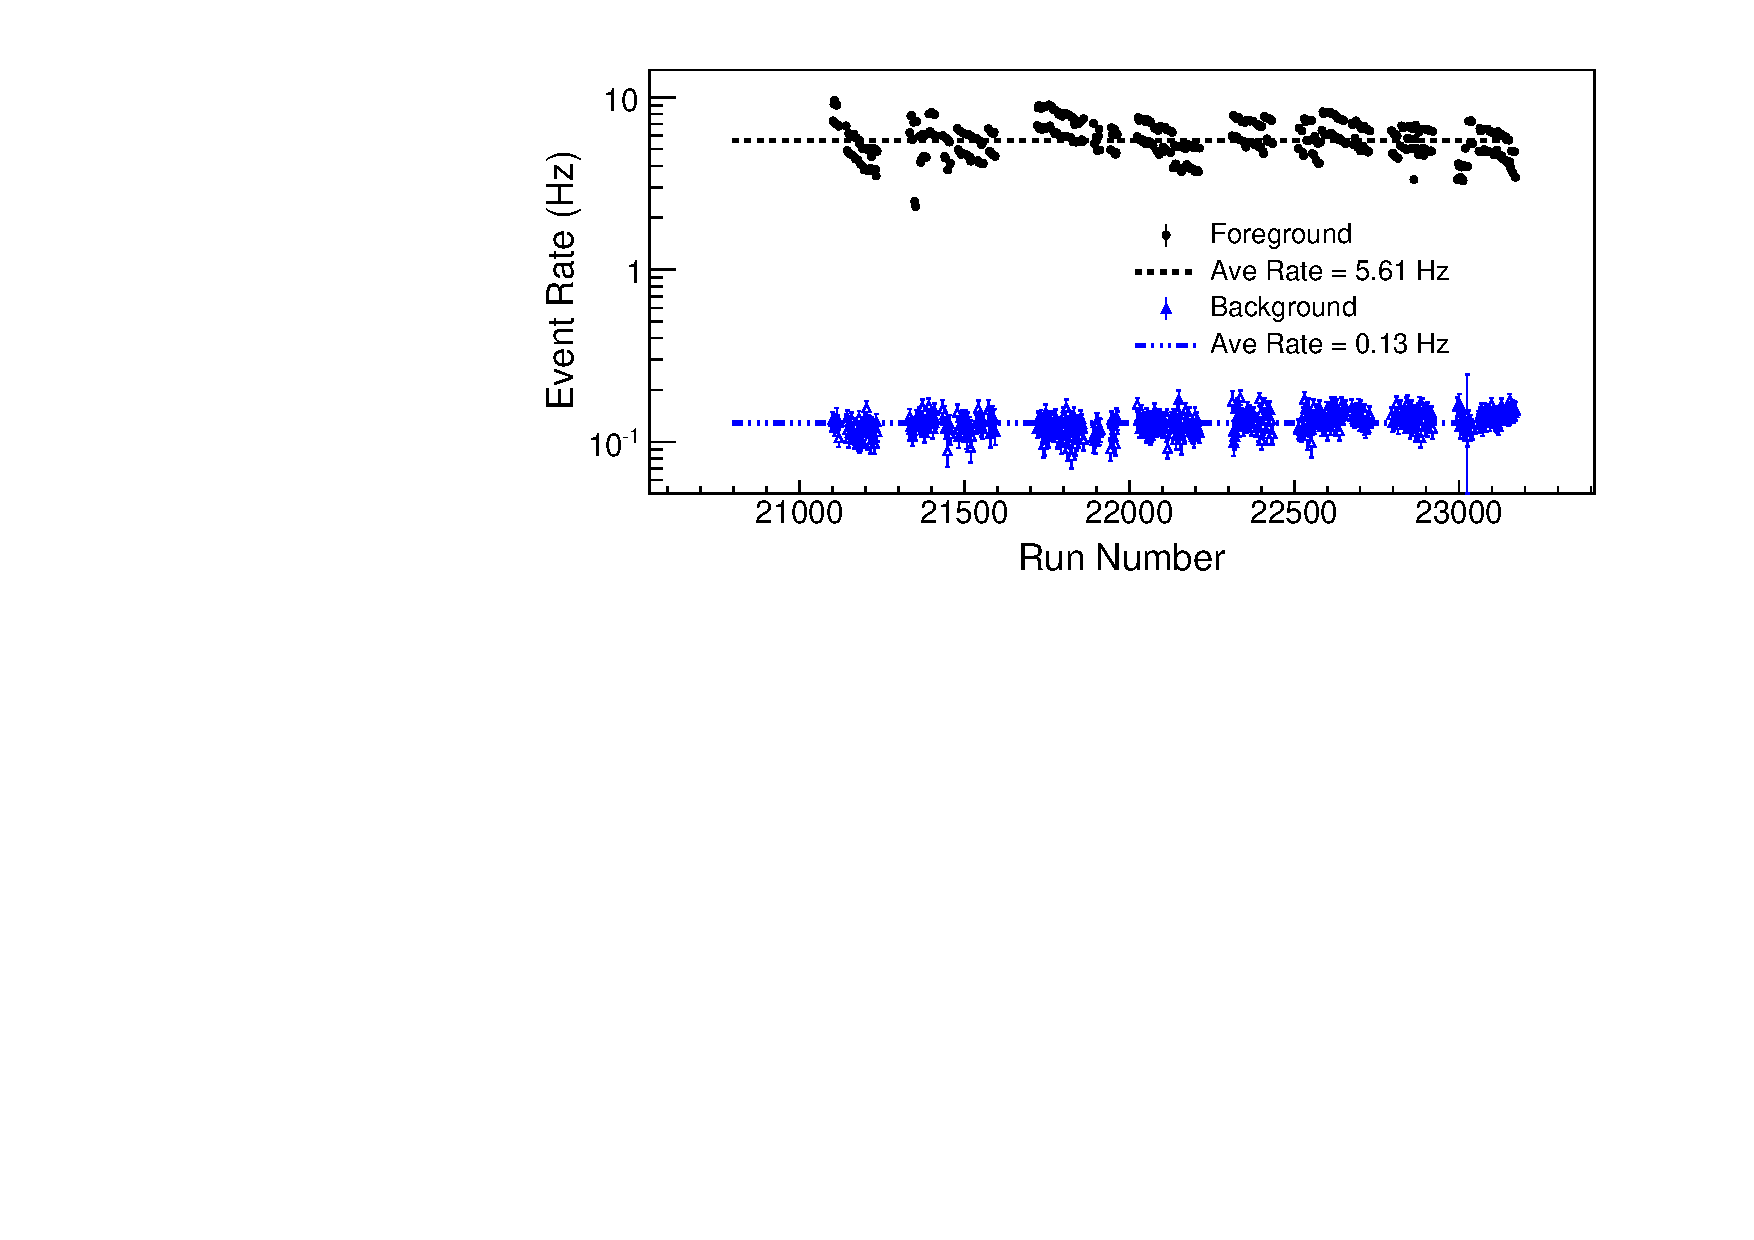
\includegraphics[page=1,scale=0.5]{5-UCNAResults/integratedRatesByRun_2012-2013_anaChC_190-740.pdf}} \\ 
    \subfloat[West Side]{\includegraphics[page=2,scale=0.5]{5-UCNAResults/integratedRatesByRun_2012-2013_anaChC_190-740.pdf}}
  \end{tabular}
  \caption{Integrated event rates for 2012-2013 East and West sides. The splitting in the
$\beta$ run rates is due to the difference between a spin-flipper ``on'' vs. spin-flipper
``off'' run, as the flipper ``on'' loading efficiency is approximately 2/3 that of
a flipper ``off'' run.}
  \label{fig:integratedRates2012}
\end{figure}

The background subtraction tranforms the rates in every bin in the following manner:
%
\begin{equation} \label{eq:bgSubtr}
  r_{\mathrm{final},i} =  \Bigg( \frac{N_{\mathrm{data},i}}{T_{\mathrm{data}}}-\frac{N_{\mathrm{bg},i}}{T_{\mathrm{bg}}} \Bigg) \pm
  \sqrt{\bigg(\frac{\sqrt{N_{\mathrm{data},i}}}{T_{\mathrm{data}}}\bigg)^2+\bigg(\frac{\sqrt{N_{\mathrm{bg},i}}}{T_{\mathrm{bg}}}\bigg)^2}
\end{equation}
%
\noindent where $r_{\mathrm{final},i}$ is the background subtracted
rate in bin $i$, $N$ refers to counts, $T$ is the total time of
a given run, and the subscipt ``data/bg'' indicates whether the
quantity comes from either the $\beta$-decay run or the
background run. Equation \ref{eq:bgSubtr} holds true
as long as the counts in both the data and background run are large enough so that
Poisson statistics may be assumed. Below some count threshold ($N<25$ for this analysis),
we resort to an estimate of the uncertainty in a given bin. To do this, we utilize
higher statistics reference spectra created by summing over all background runs for each
spin state ($\pm$) and detector side (1,2) and apply the same data selection cuts
(\ref{ssec:dataCuts}) used for asymmetry analysis. The reference spectra are essentially combinations
of those seen in figures \ref{fig:bgSpectra2011} and \ref{fig:bgSpectra2012}. The expected
background rate to be used in properly determining the background uncertainty
is then determined by multiplying the reference background fraction in some energy bin
by the total background counts in the background run, or
%
\begin{equation} \label{eq:bgRef}
  r_{\mathrm{bg},i} =  \frac{1}{T_{\mathrm{bg}}} \Bigg(N_{\mathrm{bg},i} \pm
  \sqrt{N_{\mathrm{bg,tot}} \frac{N_{\mathrm{ref,i}}}{N_{\mathrm{ref,tot}}} } \Bigg), 
\end{equation}
%
\noindent where subscript ``ref'' refers to the reference spectrum of background counts and
subscript ``tot'' refers to the integrated total counts in the respective spectrum. This new
background rate and uncertainty (note that only the uncertainty changes when $N<25$) are then
used in Equation \ref{eq:bgSubtr}. This method
removes large statistical variation in the background uncertainties when the counts
are low and gives an uncertainty
to background rates that could be zero for a given bin. 

\subsubsection{Neutron Generated Backgrounds}

Substantial work done previously by M. Mendenhall pioneered a thorough determination
of the systematic correction to $A_0$ from neutron generated backgrounds, as can be
found in \cite{mpmThesis}. Neutron generated backgrounds cannot be accounted for
using normal background subtraction as the decay trap is void of neutrons during background
runs. The correction comes mainly from UCN that escape the decay trap
and interact with other components of the apparatus. The two main mechanisms studied
were neutron capture on the aluminum wirechamber entrance and exit windows
($n+ {^{27}\mathrm{Al}} \rightarrow {^{28}\mathrm{Al}}$) and on hydrogen in
the scintillators ($n+{^{1}\mathrm{H}} \rightarrow {^{2}\mathrm{H}}$). ${^{28}\mathrm{Al}}$
subsequently $\beta$-decays (2863~keV endpoint) into an excited state of ${^{28}\mathrm{Si}}$
which emits a 1779~keV gamma upon relaxing to the ground state. The excited deuteron falls
to its ground state via emission of a 2223~keV gamma. Each of these decay products can
interact with the scintillator, so the presence of such interactions would create a small
excess of events in the
background subtracted spectra
above the $\beta$-decay endpoint, a common characteristic seen in both 2010 (used in
\cite{mpmThesis}) and in the current analysis. Since the
beyond endpoint rates agree within statistics and no changes were made to hardware outside
the decay trap, adoption of
the previously determined correction $\Delta A /A = 0.01(2)\%$ is assumed for this analysis.

\subsubsection{Veto Efficiency Uncertainty}

Gamma events and muon events that are vetoed by checking for coincidence between the scintillators and
another detector of the experiment could contribute an uncertainty to the asymmetry if the detector
used for determining a coincidence behaves erratically. If all components are fairly stable in time,
then even events which pass the veto due to inefficiency would be subtracted out using the
typical background subtraction method mentioned above. To be conservative though, the uncertainty
from the previous analysis of $\pm 0.03\%$ was applied to the final asymmetry in case of
any non-statistical fluctuations in the background rates.


\subsection{Miscellaneous Systematic Corrections and Uncertainties}

While the core Monte Carlo corrections described above make up the majority of the
simulation-motivated corrections due to effects from the aparatus, there are several
corrections and/or uncertainties determined from other Monte Carlo studies. These
systematic effects are not determined on an energy dependent basis, but rather integrated
over the final analysis window.

\subsubsection{Wirechamber Efficiency} \label{sssec:mwpcEff}

Since a dual trigger between the MWPC and the scintillator is required to differentiate between
a background gamma ray and an electron (remember the MWPC is highly insensitive to gammas),
electron events that fail to
trigger the MWPC but trigger the scintillator will be misidentified as a gamma and will not
be included in the asymmetry analysis. Higher energy, lower pitch angle events deposit less
energy in the MWPC, thus these events suffer misidentification more often
from MWPC efficiencies $<100\%$. These same
higher energy, lower pitch angle events contribute more to the
raw asymmetry as seen by rewriting Equation \ref{eq:A_SR}
and leaving the $\cos\theta$ dependence in,
%
\begin{equation}
  A_{\mathrm{SR}}=\langle P \rangle A(E) \beta \langle \cos\theta \rangle.
\end{equation}
%
\noindent Missing these events effectively decreases the measured asymmetry, thus a systematic
correction for such an effect
should act to increase the magnitude of the measured asymmetry.

The goal for determining such a correction is to use simulated data to model the effect
the efficiency of our MWPCs has on our measured asymmetry. First we need to determine
the efficiency from data. A set of long $^{113}\mathrm{Sn}$ runs with accompanying background runs
were conducted at the end of the 2011-2012 run period.
Using the background subtracted rates for MWPC triggering events (identified as an electron)
and non-MWPC triggering events (identified as a gamma ray), one can set
a lower limit on the wirechamber efficiency at the energy of the $^{113}\mathrm{Sn}$ peak
by calculating the ratio
%
\begin{equation}
  \eta_{\mathrm{MWPC}} = \frac{r_{\mathrm{trigger}}}{r_{\mathrm{trigger}}+r_{\mathrm{NoTrigger}}}.
\end{equation}
%
\noindent This is a lower limit because there could be contamination from actual gamma
rays emitted by the $^{113}\mathrm{Sn}$ source, but this contribution is quite small due
to the gammas not being confined within
the decay trap by the 1~T magnetic field and the small solid angle acceptance of the detectors
for gammas originating at the center of the decay trap. The efficiencies found were
$\eta_{\mathrm{MWPC}}=0.99912(40)$ and $\eta_{\mathrm{MWPC}}=0.99974(36)$ for the East and West
detectors respectively. 

The above efficiencies are only valid at the energy of the $^{113}\mathrm{Sn}$ source,
which is not ideal for use in the simulation as it stands.
Instead, one would
like to convert this into an energy deposition trigger threshold within the wirechamber.
Using an MWPC energy threshold rather than an efficiency
automatically creates an energy dependent efficiency, as the higher energy, lower pitch angle
electrons will deposit less energy in the MWPC and will be less likely to trigger.
Detemining the threshold is done using 
simulations of the long $^{113}\mathrm{Sn}$ runs. By scanning the MWPC threshold up from 0 keV, one can
calculate the point at which the simulated wirechamber efficiency matches the wirechamber
efficiency found using the data. The energy thresholds for the East and West
MWPCs occur at roughly 0.969~keV and 0.874~keV respectively.

At this point, the integrated asymmetry is calculated for $\beta$-decay simulations with and without
the MWPC efficiency in place, and then the correction is calculated in the usual way,
\begin{equation}
  \Delta_{\mathrm{MWPC}} = \frac{A_{\mathrm{noThresh}}}{A_{\mathrm{Thresh}}}-1, 
\end{equation}
%
\noindent where the corrected asymmetry is that without the threshold since we want to remove
the dependence on the MWPC efficiency. This was done for fifty independent batches of simulations,
and the resulting fifty corrections were histogrammed and fit with a Gaussian. The mean of this Gaussian
gives the correction, and the error on the mean gives the uncertainty.
The final $\Delta_{\mathrm{MWPC}}$ corrections are +0.13(1)\% and +0.11(1)\% for 2011-2012 and 2012-2013. 


\subsubsection{Gain Uncertainty}

Gain corrections are applied on a run-by-run basis, so variations
of the gain within each run will present themselves as an additional
energy uncertainty. To study this effect, the individual endpoint values
of every run from the data were histogrammed and the $1\sigma$ spread in
the distribution was attributed to possible uncertainty in the gain during
an individual run. Assuming that the gain is a non-energy-dependent
multiplicative factor,
one can extract the
fractional energy uncertainty for all energies by calculating the ratio
of the uncertainty at the endpoint to the endpoint energy.
The spread of the endpoint values
was determined to be $\approx 5~\mathrm{keV}$, which, upon accounting for the 782~keV endpoint
energy,
is a $0.0064\%$ uncertainty on the energy. Assuming the same constant energy
uncertainty across all electron energies and weighting by the experimentally observed
spectrum as was done in Section \ref{ssec:energyRecon}, we find uncertainties 
of $\pm0.16\%$ (2011-2012) and $\pm0.17\%$ (2012-2013) from variations in PMT gain.


\subsubsection{Magnetic Field Nonuniformity} \label{sssec:MagFieldSyst}

As shown in Section \ref{ssec:MagneticField}, the magnetic field is not uniform
near the center of the decay trap, but rather has a dip surrounded by local maxima.
Such conditions yield precarious scenarios for electrons with small longitudinal momentum
(along the decay trap axis), as electrons with total momentum $p=\sqrt{p_\parallel^2 + p_\perp^2}$
in a magnetic field $B_0$ will be reflected if encountering a local maxima $B_{\mathrm{max}}$ such that
\begin{equation}
  B_{\mathrm{max}} > B_{\mathrm{crit}} \equiv \Big( \frac{p^2}{p_\perp^2} \Big) B_0,
\end{equation}
\noindent where $B_{\mathrm{crit}}$ is the critical condition for reflection. Thus a local field maximum
will reflect a certain fraction of electrons, and a local field minimum, or field dip as
we refer to it, will trap a certain fraction
of electrons which originate within the dip.

%The potential effect of nonuniform fields on the measured asymmetry is demonstratedquantitatively in appendix \ref{app:MagField}.
Qualitatively we understand the effect on the
measured asymmetry using two ideal cases and considering the use
of the super-ratio for extracting asymmetries. We also assume we have perfect detection
efficiency in these cases.

The first nonuniformity we will consider
is a central symmetric local maximum only. By central and symmetric we mean the field profile is
identical on both sides of the maximum, which is at the center of the decay trap.
A certain fraction of electrons both to
the left and right of the maximum will be reflected back towards their initial location,
changing the detected rates in each detector. Now spin state dependent and detector dependent
acceptances nominally cancel in the super-ratio, but this modification to the rate is tied
to the distribution itself, thus its effect is seen in the measured super-ratio asymmetry.
This specific situation%, in the context of appendix \ref{app:MagField},
yields a dilution
to the asymmetry that is dependent on the magnitude of the central maximum only.

The second scenario we will consider is that of a central symmetric field minimum (field dip).
A field dip can trap $\beta$-decay electrons
that originate in the lower field region if their longitudinal momentum is
below some critical momentum, leaving them reflecting back and forth in the dip until
they scatter off of the residual gas and gain enough momentum to escape. Such a scattering
process randomizes the detected direction of the outgoing electron, thereby diluting the
asymmetry.

Each ideal scenario alone produces a dilution to the asymmetry, and one would suspect that a
correction to the asymmetry should be applied to increase the magnitude of the measured asymmetry,
but simulation has shown the potential for nonuniform fields like those we measure to create an
enhancement in the asymmetry. %This very fact led to the calculation in appendix \ref{app:MagField},
%which shows that the position and shape of a field maximum or dip can create either
%enhancement or dilution to the asymmetry.
It can be shown that an asymmetrically placed field maximum can create an enhancement to the asymmetry
which is second-order (where the expansion variable is related to the fractions of events reflected
on each side of the maximum), but the first order term produces a dilution to the asymmetry. The first-order term
is always greater in magnitude
than the second-order term when varying the position and size of the field maximum, yielding no scenario
that can produce an overall enhancement. Thus, a simple
shift of the location of the maximum cannot explain the simulation results. But, this simple calculation
does not consider that a field dip changes
the angular distribution of the electrons it traps, which in turn changes the angular
acceptance of the detected electrons, making electrons that never would have been detected before
due to high pitch angle and low energy detectable by upscattering. The field dip coupled to local maxima
on each side, which is essentially the measured field profile, is a more difficult scenario to address
in a quantitative manner, and thus we must rely on the results of the simulation.

In conclusion, the intertwined dependence of the magnetic field correction on the shapes and
positions of the nonuniformity and on the detector detection efficiencies prompted us to apply
only an uncertainty from the field nonuniformity rather than a correction. Also, we only had
reliable field data from 2011-2012, so a correction could not have been properly calculated for
2012-2013 without assumptions for the field profile. The uncertainty was
determined by choosing a typical field profile and running fifty independent simulations with and
without the field profile implemented for the 2011-2012 geometry.
Both simulations were run with an increase in vacuum
pressure from $10^{-5}$~Torr to $10^{-3}$~Torr in order to encourage upscattering from the
field dip region, otherwise electron propagation time within the dip would have been far
too computationally expensive. Since we are only studying the relative effect on the asymmetry,
such a modification is acceptable. Upon histogramming the corrections to the asymmetry from
the fifty independent simulations, one can extract the mean and error on the mean from a Gaussian
fit to the distribution, giving the mean correction to be applied of $-0.01(12)\%$, but as mentioned
we will only apply an uncertainty and no correction, so for both geometries the uncertainty from
the field nonuniformity is $\pm0.12\%$. 

In the future, the issues encountered with the present determination of the field nonuniformity
correction can be avoided. This uncertainty is strictly statistics limited, so with
larger simulations the uncertainty can be reduced. Also, if the maps are taken often (and checked
for quality), a credible time dependent correction to the asymmetry can be determined.




%--------------------------------------------------------------


\section{Theory Modifications} \label{ssec:deltaTh}

The $\beta$-decay asymmetry parameter of interest, $A_0$, is free of effects from the
recoil of the decay proton (or the daughter nucleus in the case of a nuclear decay) and
from Coulomb interactions between the charged products. What is measured
experimentally obviously includes such effects, as they cannot be disentangled simply through
observation of the decay electron momentum. The Monte Carlo corrections above are meant to correct for any geometry and
detector dependent corrections, but to resolve $A_0$, we rely on thoery calculations.

\begin{figure}[h]
  \centering
  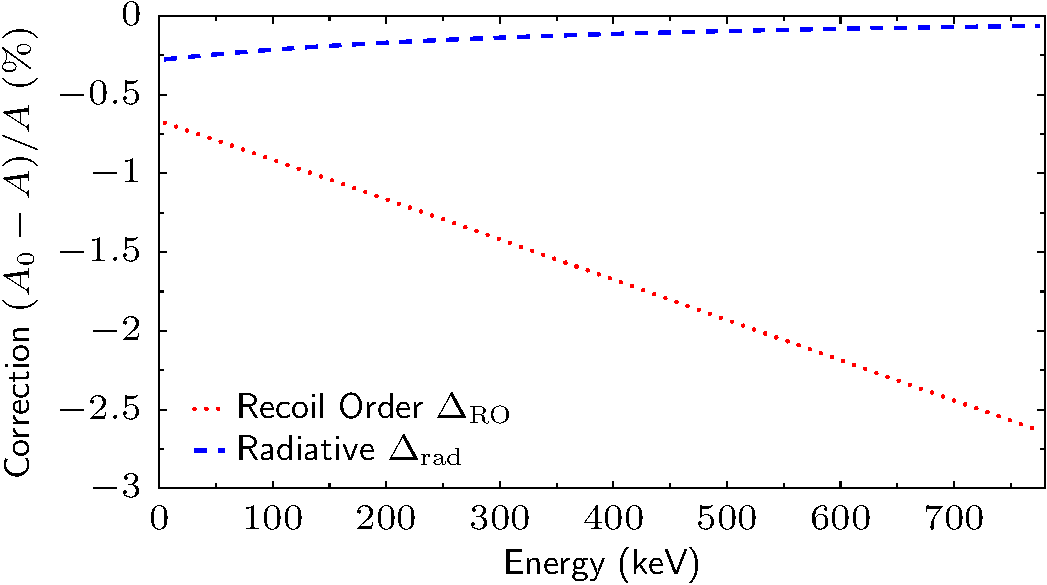
\includegraphics[scale=0.7]{5-UCNAResults/TheoryUncert2011.pdf} 
  \caption{Radiative and Recoil Order theory corrections to the measured asymmetry
  due to finite mass and non-zero charge of the final state proton.}
  \label{fig:theoryCorr}
\end{figure}

The theoretical effects come in two flavors: recoil-order modifications to address the finite
mass of the final state proton and radiative corrections to remove effects from the electron
interacting with the field of the proton. With all known systematic corrections from the experimental
setup already addressed, we can write the final extracted value of $A_0$ as
$A_0 = (1+\Delta_{\mathrm{RO}})(1+\Delta_{\mathrm{rad}})A$. The energy dependence of each
can be seen in \ref{fig:theoryCorr}.

\subsection{Recoil Order Modification $\Delta_{\mathrm{RO}}$} \label{sssec:sysROCorr}

The recoil order and weak magnetism modification
applied are those from Bilen'ki\u\i \textit{ et al.}
\cite{bilenkii1960} and further upheld by Wilkinson \cite{wilkinson1982}.
The correction takes the form 
%
\begin{multline}
  A(E) = A_0 \bigg(1+ \frac{\lambda+\mu}{\lambda\left(1-\lambda\right)\left(1+3\lambda^2\right)}\frac{1}{M}
  \Big(\lambda^2+\frac{2}{3}\lambda-\frac{1}{3}\Big)E_0 \\
  -\Big(\lambda^3+3\lambda^2+\frac{5}{3}\lambda-\frac{1}{3}\Big)E
  +\Big(2\lambda^2\left(1-\lambda\right)\Big)\frac{1}{E}\bigg),
\end{multline}
%
\noindent where $E$ is the electron total energy, $E_0$ is
the endpoint energy of the electron, $\lambda\equiv\frac{g_A}{g_V}$,
$M$ is the neutron mass,
and $\mu\equiv\mu_p-\mu_n$.

%The correction is reported at the 0.001\%
%level on $\lambda$, or roughly 0.004\% on $A_0$ \cite{wilkinson1982}.

The correction to the asymmetry, when integrated over the analysis window
and weighted by statistics, is -1.68(3)\% and -1.67(3)\% for 2011-2012 and
2012-2013 respectively. The uncertainties are conservative and carried over
from the previous analysis.

It should be noted that the formalism above includes only the usual vector and
axial vector terms in the hadronic current, as well as the weak magnetism
coupling. Other work form Gardner and Zhang
\cite{gardner2001}, as discussed in Section \ref{sssec:ROCorr}, includes all potential interaction terms.
The results agree with those from Bilen'ki\u\i \textit{ et al.} and Wilkinson when the second class terms
are neglected. 

\subsection{Radiative Modification $\Delta_{\mathrm{rad}}$} \label{sssec:sysRadCorr}

Sirlin first calculated the $O(\alpha)$ corrections to the unpolarized neutron
$\beta$-decay electron energy spectrum \cite{sirlin1967}, followed a few years
later by Shann's \cite{shann1971} extension of the formalism for polarized neutrons. The asymmetry is
modified by the amount $\big(1+\frac{\alpha}{2\pi }(h-g)\big)$, or
%
\begin{equation}
  A(E) = A_0\bigg(1+\frac{\alpha}{2\pi}\Big(h(E,E_0)-g(E,E_0)\Big)\bigg),
\end{equation}
where
\begin{multline}
  h-g = 4 \bigg( \frac{E_0-E}{3E\beta^2} \bigg)
  \bigg( \frac{\tanh^{-1}\beta}{\beta}-1 \bigg)
  \bigg(1-\beta^2+ \frac{E_0-E}{8E} \bigg) \\
  + \frac{\tanh^{-1}\beta}{\beta}
  \bigg( 2-2\beta^2-\frac{\left(E-E_0\right)^2}{6E^2} \bigg).
\end{multline}
%
\noindent $E$ and $E_0$ are the electron energy and endpoint energy, and
$\beta\equiv v/c$. The correction over the analysis energy window
is -0.12(5)\% for both 2011-2012 and 2012-2013.


%---------------------------------------------------------------------------

\section{Final Asymmetries}

The last step in determining the asymmetry parameter is, of course, extracting the
asymmetry from the $\beta$-decay data. Application of all described Monte Carlo
corrections and uncertainties to the measured asymmetry produces a value for
$A_0$ and thereby determines the ratio of the axial vector to vector coupling
constants in the weak interaction, $\lambda \equiv \frac{g_A}{g_V}$.

The general process includes choosing the proper subset of our data for the
asymmetry extraction, making analysis cuts, optimizing our final analysis energy
window to minimize uncertainties, and finally unveiling the result. This section
is dedicated to these steps.

\subsection{Blinding}
All of the analysis discussed up until this point, and even all stages of the
asymmetry extraction up until revealing the final result,
are completed using blinded data, making this entire
analysis a blind analysis. The idea behind blind analyses
is to introduce a bias to your data in some way
that would not allow anyone to know the final answer during all systematic studies. This
removes the human temptation to skew corrections in such a way that the new result
converges towards a personally desired result. This could be an attempt to achieve agreement
with previous results or to move further from a null hypothesis to achieve discovery.
Either way, avoiding this temptation makes for better science.

For this analysis, blinding was achieved by modifying the time stamps of every event
in such a way that the the blinding factor (as part of the
detector rates) would not cancel in the super-ratio. This required
altered time stamps which are spin-state and detector
dependent and do not cancel in the super-ratio. We produce two independent
random blinding factors, $f_{1,2}$, such that
%
\begin{equation}
  t^{\pm}_{1,2} = (1 \pm f_{1,2}) \cdot t
\end{equation}
%
\noindent where $t$ is the global time
and $t^{\pm}_{1,2}$ are the blinded times for each detector in each spin state. We completed
detector calibrations, all systematic corrections, and the polarimetry analysis prior to
unblinding, at which point all rates were recalculated using the proper global time $t$,
generating the final unblinded asymmetries.

\subsection{Data Selection and Processing}

The data selection step generally involves choosing events that are ``good'' electron
events, trying to preserve as many as possible to increase the statistical power while avoiding
unforeseen systematic effects from questionable events. These cuts are also applied to
the simulated data when determining systematic corrections for consistency. Thus, if the
model appropriately accounts for all experimentally induced deviations from the ideal
asymmetry, the asymmetries from data and Monte Carlo should be consistent.

\subsubsection{Cuts} \label{ssec:dataCuts}% Discuss position and timing cuts, also beam drops

The first cut applied is a fiducial cut
selecting events within $50$~mm of the center of the decay trap. The fiducial cut removes
events that could have potentially interacted with the decay trap wall, as the
maximum radius of the electron's spiral around the magnetic field is 7.76~mm and the wall
of the decay trap is 62.2~mm from the center. Interactions with the walls of the decay trap
can modify the energy and direction of the electron, thereby affecting the measured
asymmetry. While the Monte Carlo model should be able to correct for this, avoiding the
interactions altogether is advantageous.

We also remove from data and background runs
any events that occur when the proton beam is dropped, which means no neutrons
are being produced. Since we use the rate over an entire run in the super-ratio,
using time periods with few events reduces the average rate. The real issue with this comes
from the background subtraction, which is meant to account for backgrounds that could stem
from beam related interactions. If either the $\beta$-decay or background run has a
highly disproportionate amount of run time with the proton beam missing, the background
subtraction for that run is not as effective. To illustrate this effect, imagine a background
run where the proton beam was off for its entirety. The beam related background would thus be
``zero'' for the $\beta$-decay run that accompanies this background run, and the subsequent
subtraction of the background run would leave the $\beta$-decay rates unaffected.
While the extreme case is never observed, it is useful to remove
periods of the runs where the proton beam is missing. A running monitor of the UCN production is
used to determine when to cut intervals of data, dropping the events when the UCN rate
in UCN Monitor 1 (the first monitor beyond the UCN source) falls below 2~Hz.
The rate for all data was generally $>20$~Hz.
Any events that occur within 0.05~s of the proton beam burst are also cut to improve
the signal to background ratio.

Two wirechamber cuts, beyond the position cut, were also applied. The first is a cut on the ``shape''
of the wirechamber signal based on an algorithm developed by a collaborator C. Swank from Caltech.
By shape we simply mean what the collection of cathode ADC signals look like when plotted as a
function of position.
While the
algorithm classifies events as one of eight shapes based on the magnitude of
the signal on each wire group, the cut is used to remove non-physical shapes
like multiple positions in one wirechamber. The second wirechamber
cut simply checks that at least one cathode wire group in each plane was above threshold
so that a position can be assigned to that event.
Since a model of the cathode response was
developed for the Monte Carlo in this analysis, these same cuts could be applied to the
simulation to account for any systematic effect if these events are not simply random.

The last cut applied is an energy cut where we check that each event lies within the
energy range $190\mathrm{~keV} < T_e < 740\mathrm{~keV}$.
Within this energy range, the events are further separated into
10~keV energy bins for energy dependent asymmetry extraction. The determination
of this analysis energy window is described below in Section \ref{ssec:enRange}.
All asymmetries shown from now on
will be fit or integrated over this energy range.

\subsubsection{Data Taking Structure}

For use of the super-ratio technique, one must use at least two runs with differing loaded
neutron spin states. For the UCNA experiment, we use what we call an octet data structure,
consisting of eight $\beta$-decay runs, eight background runs, and eight depolarization
runs, with the spin-state changing in such a way that produces
four runs from each $\pm$ spin state.
The details of this method can be found in \cite{plaster2012}. This method allows for
construction of three different super-ratio asymmetries: octet asymmetries (utilizing all eight background subtracted
$\beta$-decay runs in the asymmetry), quartet asymmetries (using four consecutive spin-flipped
runs in the asymmetry), and pair asymmetries (using two consecutive spin-flipped runs). Each octet can potentially
produce four pair asymmetries and two quartet asymmetries. We use
the octet asymmetries in the extraction of the final asymmetry, as this structure lends to more
efficient cancellation of time varying backgrounds. Figure \ref{fig:RawAsymms} shows the
raw asymmetries extracted from all three types of data groups. The results are consistent
within statistical uncertainties, and the $\chi^2/\textrm{NDF}$ indicates the fluctuations
are statistical. 

\begin{figure}
  \centering
  \subfloat[Pair Asymmetries]{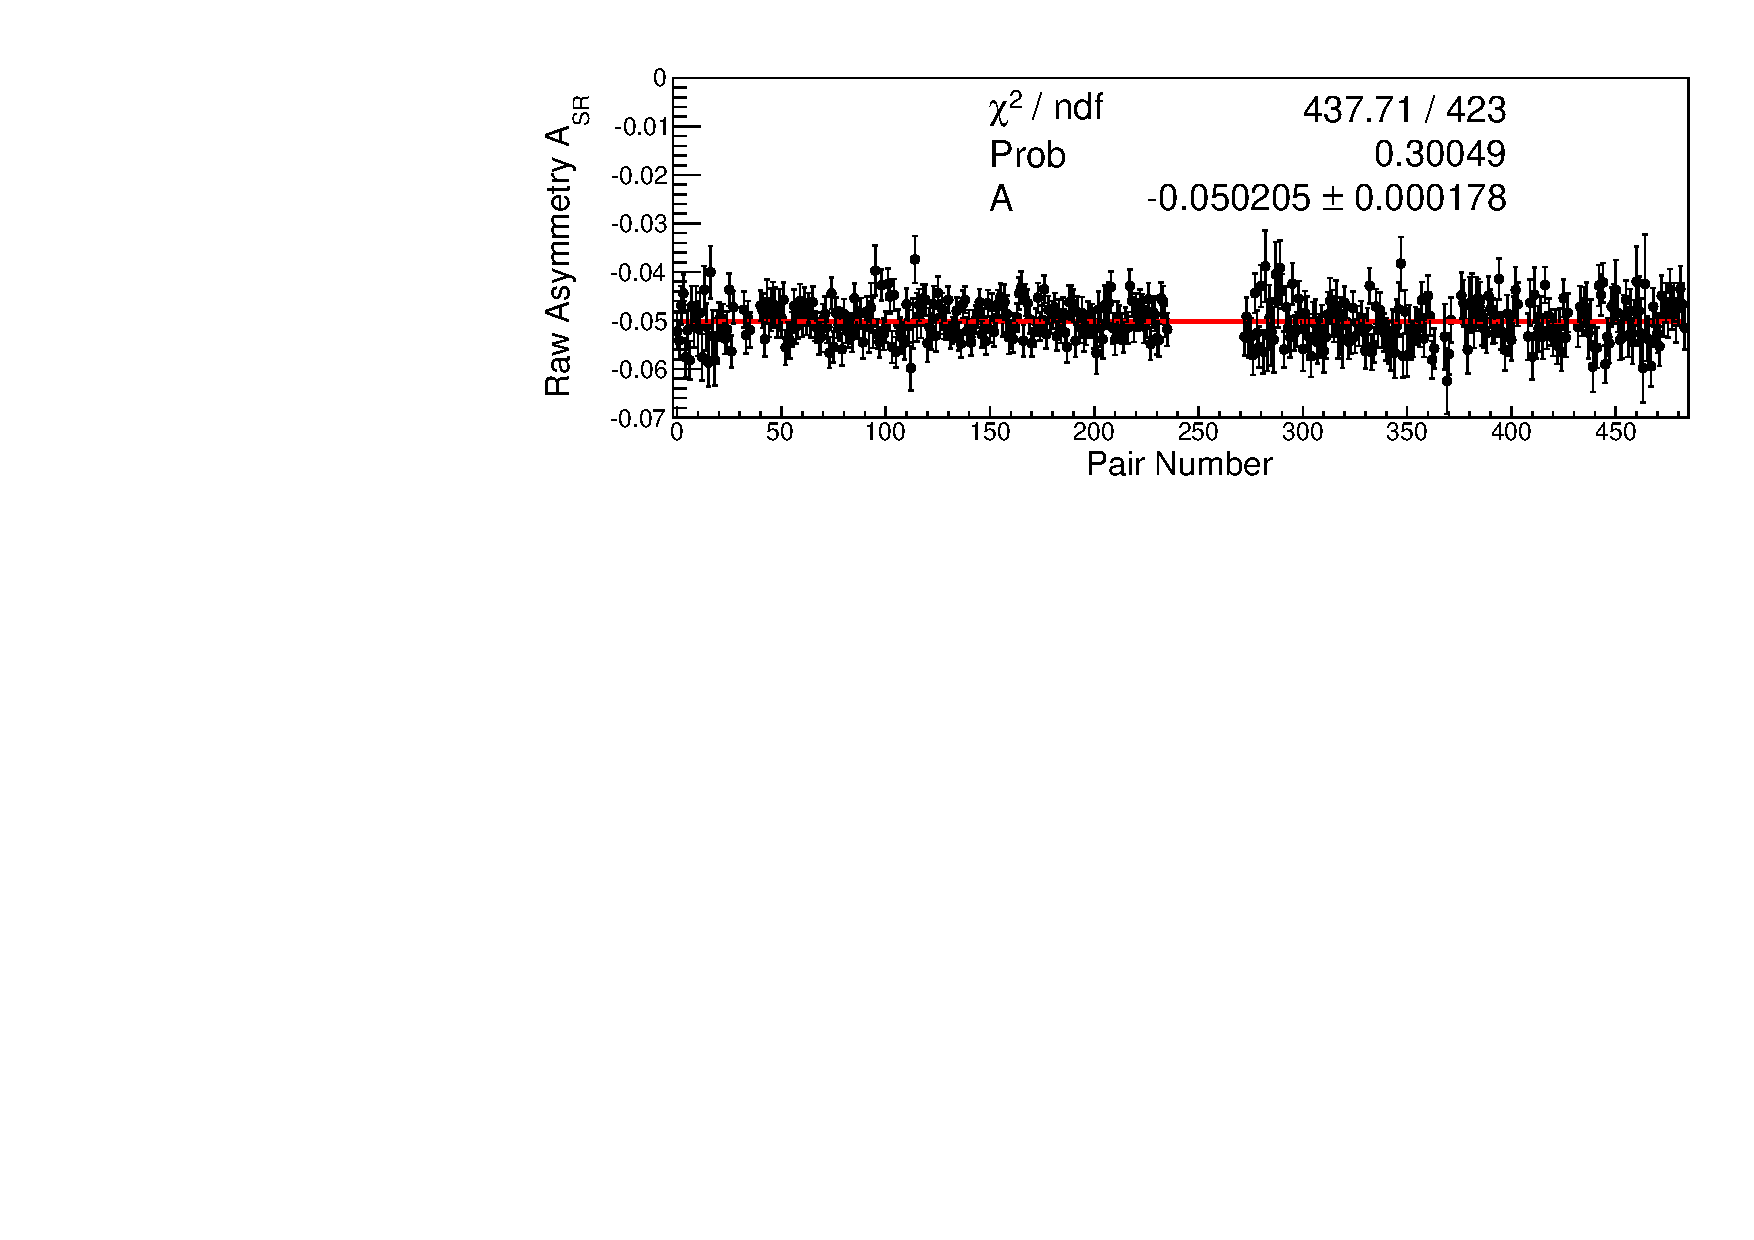
\includegraphics[page=1,scale=0.5]{5-UCNAResults/UnCorr_PairAsymmetries_AnaChC_190-740_Octets_0-121.pdf}} \\
  \subfloat[Quartet Asymmetries]{\includegraphics[page=1,scale=0.5]{5-UCNAResults/UnCorr_QuartetAsymmetries_AnaChC_190-740_Octets_0-121.pdf}} \\ 
  \subfloat[Octet Asymmetries]{\includegraphics[page=1,scale=0.5]{5-UCNAResults/UnCorr_OctetAsymmetries_AnaChC_190-740_Octets_0-121.pdf}} 
  \caption{All raw super-ratio asymmetries as a function of group number, whether octet, quartet, or pair.
    There are no systematic corrections applied, and the asymmetries are integrated over the analysis window 190-740~keV.
    The split in the data is a batch of data from 2012-2013 that had to be discarded due to bad timing information.}
  \label{fig:RawAsymms}
\end{figure}

\subsubsection{Analysis Choices} \label{sssec::anaChoices}

We have identified four detected electron event types thus far in this analysis, namely Type 0, 1,
2, and 3. In summary, Type 0 events are those which are identified as single detector events, meaning they
trigger one detector package only, and they make up almost 95\% of detected events. Types 1, 2, and 3
are identified as backscattering events, with Type 1 events triggering both scintillators, while 2 and 3
trigger both wirechambers but only one scintillator. Based on solely trigger logic, a Type 2 cannot be
distinguished from a Type 3, but a delineation can be made between them given their energy deposition
in the MWPC. See Section \ref{sec:backscattering} for a detailed description of the backscattering events and
Section \ref{sssec:backscSep} for implementation of the MWPC calibration used to separate the Type 2 and Type 3 events.

\begin{figure}[h]
  \centering
  \subfloat[2011-2012]{\includegraphics[page=1,scale=0.70]{5-UCNAResults/CorrVsUncorr_singleAxis_color.pdf}} \\
  \subfloat[2012-2013]{\includegraphics[page=2,scale=0.70]{5-UCNAResults/CorrVsUncorr_singleAxis_color.pdf}} 
  \caption{Asymmetries for different subsets of data. The * signifies unseparated Type 2 and Type 3 events.
    The inset shows the asymmetries that include Type 0 events, as the uncertainties
    are too small to see in the main figure. The only corrections applied to these asymmetries are
    the energy dependent Monte Carlo corrections and the polarization correction. The error bars are
    purely statistical, so the observed agreement between asymmetries is a lower limit.}
  \label{fig:anaChAsymms}
\end{figure}

Inclusion of any subset of the aforementioned event types in the analysis produces different
asymmetries, where any choices that
have like event types are correlated at the level of the fractional statistical uncertainty of the like
types. One may also decide to include the Type 2/3 events as unseparated or separated by the MWPC energy
cut, giving yet another set of analysis choices. For this analysis, we used all event types with the
Type 2 and Type 3 separated. This choice utilizes maximal statistics, while separating the Type 2/3 events
requires smaller systematic corrections and uncertainties than leaving them unseparated.

Figure \ref{fig:anaChAsymms} shows the asymmetries for all analysis choices considered, with the
event types included in the asymmetry extraction listed on the horizontal axis. There is a
noticeable improvement in the agreement across all analysis choices compared to previous analyses,
indicating improvement in the Monte Carlo corrections, namely $\Delta_2$ and $\Delta_3$.
The uncertainties in the figure are
purely statistical, so the agreement seen is a worst case scenario as inclusion of systematic uncertainties
inflates the error bars. 

\subsection{Determining $A_0$}


\subsubsection{Combining Results} \label{sssec:comboResult}

After selecting the data to be used in the final determination of the asymmetry, one is left with
two separate blinded results, one from each geometry (2011-2012 and 2012-2013). The results
are then combined via a method developed for the previous analysis by M. Mendenhall
\cite{mpmThesis}. In summary, the combination is a modified weighted average that takes into
account correlations between all uncertainties. Uncorrelated uncertainties will improve
the final uncertainty, while correlated uncertainties cannot. The method inherently solves for
the weighting factors that minimize the total uncertainty of the combined final result.

For this analysis, the individual systematic uncertainties from each geometry (i.e. $\Delta_2$ from
2011-2012 and 2012-2013)
are taken to be completely correlated, but they are uncorrelated with all other uncertainties.
The statistical uncertainty of one geometry is the only uncertainty treated as
uncorrelated with its counterpart from the other geometry, as we would like to take advantage of
the combined statistical power of each result. 

\subsubsection{Optimization of energy range} \label{ssec:enRange} % maybe remove this and just discuss it

Once the framework for combining results is in place, the energy analysis window must be determined.
Ideally, the analysis window should be one that minimizes the total uncertainty given the subset of data chosen
for the final result, but, because several of the integrated corrections require the analysis window
as input, we only consider the uncertainties from statistics, energy reconstruction,
and energy dependent Monte Carlo corrections during minimization.

\begin{figure}[p]
  \centering
  \subfloat[Statistical Uncertainty]{\includegraphics[page=1,scale=0.4]{5-UCNAResults/TwoDimUncert.pdf}} \\
  \subfloat[Systematic Uncertainty (Combined Energy Uncertainty and Monte Carlo uncertainty)]{\includegraphics[page=2,scale=0.4]{5-UCNAResults/TwoDimUncert.pdf}} \\
  \subfloat[Combined systematic and statistical uncertainty]{\includegraphics[page=3,scale=0.4]{5-UCNAResults/TwoDimUncert.pdf}} \\ 
  \caption{Plots of the fractional uncertainty on the extracted asymmetry for given minimum and maximum limits
    on the analysis window. The minimum of the combined systematic and statistical uncertainty is used for the
    final analysis window, $190\mathrm{~keV} < T_e < 740\mathrm{~keV}$.}
  \label{fig:enWindow}
\end{figure}


\begin{figure}[h]
\centering
\includegraphics[page=6,scale=.5]{5-UCNAResults/TwoDimUncert.pdf}
\caption{Statistical and systematic errors used in minimization of the energy window. This is a projection
  of Figure \ref{fig:enWindow} about the minimum window cut of 190~keV to show the dependence on energy cut
  more effectively.}
\label{fig:enWindow1D}
\end{figure}

\begin{figure}[h]
  \centering
  \subfloat[$\frac{A-A_{\mathrm{min}}}{\delta A}$]{\includegraphics[page=4,scale=.5]{5-UCNAResults/TwoDimUncert.pdf}} \\
  \subfloat[Plot of $1\sigma$ agreement]{\includegraphics[page=5,scale=.5]{5-UCNAResults/TwoDimUncert.pdf}}
  \caption{Panel (a) shows the ratio of $(A-A_{\mathrm{min}})$ to $\delta A$, where $\delta A$ is the $1\sigma$ total uncertainty
  taken from Figure \ref{fig:enWindow} panel (c). The $z$-axis is a measure of agreement between
  the asymmetry in a bin with the overall minimum uncertainty bin, $A_{\mathrm{min}}$, in units of $\sigma$ of
  the bin being used. Values between $-1$ and $+1$ indicate that the asymmetry in the bin is in agreement with
  $A_{\mathrm{min}}$ at the $1\sigma$ level. Panel (b) shows the bins for which this $1\sigma$ agreement is met. The black
  circle in each figure indicates the location of $A_{\mathrm{min}}$.}
\label{fig:enWindowAsymm}
\end{figure}

The final energy window is calculated by scanning all possible energy windows in
10~keV increments, with a minimum lower bound at
$>100$~keV and a maximum upper bound of $<780$~keV. The total width of the energy window
is set to start at 100~keV to save on computation
time but is not limited beyond that. Upon exploring all energy windows, the minimum combined uncertainty
occurs at $190\mathrm{~keV} < T_e < 740\mathrm{~keV}$ shown.
Figure \ref{fig:enWindow} shows the uncertainty contributions as a function of energy window. The
final plot shows the combined uncertainty from all three contributions, and we
see that the window $190\mathrm{~keV} < T_e < 740\mathrm{~keV}$ falls within the area
of the minimum uncertainty. Once we choose the minimum edge of our window, we can view the
dependence of the final uncertainty as a function of the upper edge of the analysis window
as seen in Figure \ref{fig:enWindow1D}. Here we see the total uncertainty becomes essentially
constant beyond an upper window cut of 690~keV.
The dependence of the asymmetry on energy window can be seen in Figure \ref{fig:enWindowAsymm} panel (a),
where the ratio $(A-A_{\mathrm{min}})/\delta A$ is plotted. The asymmetry is consistent with the
minimum energy window asymmetry ($A_{\mathrm{min}}$) within
a $1\sigma$ uncertainty over a large portion of the sampled analysis windows. Figure
\ref{fig:enWindowAsymm} panel (b) shows all of the energy windows that produce a $1\sigma$ agreement.
The minimum energy window chosen is indicated in the figure by the black dashed circle, well within
a region where the asymmetry is stable.


\subsubsection{Unblinded Result}

\begin{figure}[h]
  \centering
  \includegraphics[scale=0.4]{5-UCNAResults/SuperSumTotal.pdf} 
  \caption{Final beta decay spectrum from data (open circles), Monte Carlo (solid line),
    and the subtracted background (closed circles). The bottom shows the difference between the
    Monte Carlo spectrum and the data.}
  \label{fig:FinalSpectrum}
\end{figure}

\begin{figure}[h]
  \centering
  \subfloat[2011-2012 Asymmetry with energy dependence ($\frac{\beta}{2}A_0$)]{\includegraphics[page=1,scale=0.38]{5-UCNAResults/asymm_2011-2012.pdf}} 
  \subfloat[Final 2011-2012 $A_0$]{\includegraphics[page=2,scale=0.38]{5-UCNAResults/asymm_2011-2012.pdf}} \\
  \subfloat[2012-2013 Asymmetry with energy dependence ($\frac{\beta}{2}A_0$)]{\includegraphics[page=1,scale=0.38]{5-UCNAResults/asymm_2012-2013.pdf}}  
  \subfloat[Final 2012-2013 $A_0$]{\includegraphics[page=2,scale=0.38]{5-UCNAResults/asymm_2012-2013.pdf}} 
  \caption{Final unblinded 2011-2012 and 2012-2013 asymmetry with all systematic corrections applied. The dashed line in
    a.) and c.) uses PDG $A_0=-0.1184$ for comparison. The fits in b.) and d.) are over the
    final analysis window, $190\mathrm{~keV} < T_e < 740\mathrm{~keV}$. The uncertainties are statistical only.}
  \label{fig:FinalA}
\end{figure}

\begin{figure} [h]
  \centering
  \includegraphics[scale=0.7,page=1]{5-UCNAResults/ucna_2017.pdf}
  \caption{Historical plot of $A_0$ measurements including the measurement resulting from this analysis
    \cite{bopp1986,erozolimskii1991new,yerozolimsky1997,liaud1997,abele2002,mund2013,mendenhall2013,brown2017}.
    The shaded band indicates the Particle Data Group average value \cite{pdg}
    for the asymmetry parameter, where the solid data points are included in the average (not including
    the Brown \textit{et al.} point, as this will be included in future averages). Figure credit: Dr. Brad Plaster
    \cite{bradPlot}}
  \label{fig:AmeasurementsNew}
\end{figure}

On August 16, 2017, upon completion of all systematic studies and the asymmetry analysis code, the data
was unblinded and the asymmetries recalculated using the proper time stamps. The energy dependent asymmetries
and final asymmetries for the two geometries, 2011-2012 and 2012-2013, are shown in Figure \ref{fig:FinalA},
with fits over the final analysis window of $190\mathrm{~keV} < T_e < 740\mathrm{~keV}$.
The unblinded asymmetries with both statistical and systematic uncertainties accounted for
are $A_0=-0.12026(54)_{\mathrm{stat}}(67)_{\mathrm{syst}}$ and $A_0=-0.12111(74)_{\mathrm{stat}}(69)_{\mathrm{syst}}$
for 2011-2012 and 2012-2013 respectively.
Utilizing the method described in section
\ref{sssec:comboResult} for combining results, the 2011-2012 and 2012-2013 asymmetries were combined
with weights of 0.67 (2011-2012) and 0.33 (2012-2013), yielding a final value of
$A_0=-0.12054(44)_{\mathrm{stat}}(68)_{\mathrm{syst}}$ corresponding to a
value for the ratio of the axial-vector to vector coupling constants of
$\lambda\equiv \frac{g_{A}}{g_{V}}=-1.2783(22)$, where the statistical and systematic
uncertainties have been added in quadrature. Figure \ref{fig:AmeasurementsNew} shows schematically
where the present result lies in comparison to previous measurements of $A_0$. 

We also report a combined result using our previous measurement \cite{mendenhall2013} and a
similar weighting method as above, only now we set all systematic uncertainties
to the smallest reported value between the two measurements and treat them as completely correlated.
This in turn means we do not benefit beyond the best measurement of any systematic uncertainty, but
that we take advantage of the increased statistics. This culminates in the combined UCNA results of
$A_0=-0.12015(34)_{\mathrm{stat}}(63)_{\mathrm{syst}}$ 
and $\lambda\equiv \frac{g_{A}}{g_{V}}=-1.2772(20)$, with weights of 0.39 for the previous
result \cite{mendenhall2013} and 0.61 for the result from this analysis.


\section{Future Outlook for UCNA and $A_0$ Measurements}
% include plot of Vud crossing, but add new Perkeo measurement if it has been released
% Talk about UCNA+

While this measurement concludes results for $A_0$ from the UCNA experiment in its current
capacity, there are hopes for a next generation UCNA$+$ experiment. The uncertainties described
within this thesis, namely the backscattering, $\cos\theta$, and energy reconstruction
uncertainties,  limit the UCNA Experiment as currently configured to the present precision.

\begin{figure}[h]
\centering
\includegraphics[scale=.7]{5-UCNAResults/vud_vs_lambda_color.pdf}
\caption{Status of $V_{ud}$, the neutron lifetime, and $\lambda$
  measurements. The $\lambda$
  result bands (vertical) are divided into pre-2002 \cite{bopp1986,yerozolimsky1997,liaud1997}
  and post-2002 \cite{mostovoi2001,schumann2008,mund2013,mendenhall2013}
  results, where the distinction is made using the date of the
  most recent result from each experiment. The right axis
  shows publication year for the individual lambda measurements 
  included in the calculation of the $\lambda$ bands (closed markers for post-2002,
  open markers for pre-2002). Note that the result of this work (Brown \textit{et al.})
  is the combined UCNA result from \cite{mendenhall2013} and the current analysis, and the
  Mund \textit{et al.} result is the combined PERKEOII result from \cite{abele2002,mund2013}.
  The diagonal bands
  are derived from neutron lifetime measurements 
  and are separated into neutron beam \cite{yue2013,byrne1996} and UCN bottle
  experiments, which consist of material bottle storage \cite{serebrov2005,
    arzumanov2015,steyerl2012,pichlmaier2010,mampe1993} and magnetic bottle storage \cite{pattie2017}.
  The $V_{ud}$ band (horizontal) comes from
  superallowed $0^+ \rightarrow 0^+$ nuclear $\beta$-decay
  measurements \cite{pdg}. The error bands include scale factors
  as prescribed by the Particle Data Group \cite{pdg}.}
\label{fig:vud_vs_lambda}
\end{figure}

With this in mind, UCNA$+$ intends to take actions to drastically reduce
$\Delta_3$, or the $\cos\theta$ correction, which can be achieved by decreasing the fraction
of electrons that are lost due to inefficiencies within the spectrometer. These mainly come from
the existence of the foils at the end of the decay trap, so the idea is to remove the foils and no longer
confine the neutrons within the decay volume. With
the recent upgrades in the UCN source performance, trapping the neutrons within the decay volume is
less important than it was during previous UCNA runs. Another interesting proposal is to have annular
endcaps with a hole in the middle. This would allow one to make a radial position cut on the electron
events to use events which either originated in the region with effectively no endcap or in the outer
region where the electron would see an endcap. Comparisons between these two types of events sheds
light on the behavior of the correction from data itself, and when compared to Monte Carlo can help
determine the level at which the Monte Carlo corrections are accurate. This comparison with Monte Carlo
may improve both the backscattering and $\cos\theta$ systematic uncertainties.

As for the energy reconstruction, detectors with better linearity and perhaps a
self-position-reconstructing scintillator would be useful. With position reconstruction accomplished
within the scintillator, the wirechambers could be removed thus reducing the $\cos\theta$ correction
further. Another potential improvement, although admittedly difficult,
would be the development of a calibration method
which samples the entire fiducial volume, or at least a larger fraction of the detector face. The activated
xenon spectrum highlights the promise of such a method, as it fills the entire specrometer during position
map calibration runs, but the existence of discrete conversion lines within the calibration gas would create
a completely determined calibration for every ``pixel'' of the detector. This would remove the need for position
maps altogether and would avoid any
potential bias from measuring the position dependence of the detector with a characteristic of the xenon
spectrum that is beyond the endpoint of the electron spectrum, an imperfect method when the detector
shows any non-linear behavior. Obviously a method like this, especially one that fills the entire
spectrometer rather than just the decay trap, would require systematic studies of its own.

The future of $A_0$ and $\lambda$ measurements is quite promising given the status of recent results. Figure
\ref{fig:vud_vs_lambda} illustrates the current dilemma facing the experimental nuclear physics community regarding
weak interactions and the neutron itself.
Of measurements included in the current 2017 Particle Data Group (PDG) average, 
there is a several $\sigma$ discrepancy between $\lambda$ measurements prior to 2002 and those
after 2002. One also sees from the figure that a similar splitting of neutron lifetime values has occurred,
with the difference seemingly arising between experiments using neutron beams \cite{yue2013,byrne1996}
and those using UCN (both
material bottle \cite{serebrov2005,arzumanov2015,steyerl2012,pichlmaier2010,mampe1993}
and magnetic bottle \cite{pattie2017} measurements). When combined with measurements of the CKM
matrix element $V_{ud}$ from superallowed $0^+\rightarrow 0^+$ nuclear $\beta$-decays, a clearly favorable
scenario presents itself, and further precision measurements of both $\lambda$ and $\tau_n$ will assist
in settling the matter.

The older pre-2002 measurements of $\lambda$ prompt the PDG to apply a scale factor of 2.2 to the uncertainty
on the global average for $\lambda$ (and a scale factor of 2.4 to $A_0$).
The PDG only includes in
the calculation of the scale factor those measurements that satisfy
\begin{equation}
  \delta x_i < 3 \sqrt{N} \delta \bar{x},
\end{equation}
\noindent where $x_i$ refers to one measurement of quantity $x$ out of $N$ measurements and
$\delta \bar{x}$ is the non-scaled error on the weighted average $\bar{x}$ \cite{pdg}. So while
the older measurements carry very little weight in the average value and the non-scaled uncertainty,
they drastically affect the $\chi^2$. One solution to this issue is to improve the uncertainty on
modern $A_0$ and $\lambda$ measurements, as inclusion of a 0.1\% result for $A_0$ (yielding a 0.025\% result for
$\lambda$), removes the pre-2002 results for $\lambda$
from those that enter the calculation of the
scale factor. An expected result from PERKEOII is expected to have an
uncertainty $<0.3\%$ on $A_0$, and hopefully a next generation
UCNA$+$ experiment can contribute the disired precision to remove the scale factor from the PDG average values
for $A_0$ and $\lambda$ altogether.















